%%%*******************************************************************************
%  Classe Latex SENAI CIMATEC, Version 0.0.0 16/04/2009
%
%  Define as normas e estilo das dissertaes e teses do SENAI CIMATEC
%
%  Author : Hernane Pereira
%%%-------------------------------------------------------------------------------

%%%-------------------------------------------------------------------------------
% Changes log
%%%-------------------------------------------------------------------------------
% Version 1.1.1 - 08/03/2005
% - Added support for amsmath, amsthm, amsfonts and amssymb as default
%
% Version 1.1.0 - 22/07/2004
% - updated university front page format
%
% Version 1.1.0 - 20/06/2003
% - Initial version
%%%-------------------------------------------------------------------------------

%%%-------------------------------------------------------------------------------
%  DOCUMENTATION WITH EXAMPLE
%%%*******************************************************************************

%%%-------------------------------------------------------------------------------
%%% Thesis default options
%%%-------------------------------------------------------------------------------
%\documentclass[subook]{Classes/PPGMCTI}
%\documentclass[sureport]{Classes/PPGMCTI}

%%%-------------------------------------------------------------------------------
%%% Thesis custom options
%%%-------------------------------------------------------------------------------

%%% Fancy page headings
%\documentclass[fancyheadings, subook]{Classes/PPGMCTI}
%\documentclass[fancyheadings, sureport]{Classes/PPGMCTI}

%%% Fancy chapters and sections headings
%\documentclass[fancychapter, subook]{Classes/PPGMCTI}
%\documentclass[fancychapter, sureport]{Classes/PPGMCTI}

%%% Fancy page , chapters and sections headings
%\documentclass[fancyheadings, fancychapter, subook]{Classes/PPGMCTI}
%\documentclass[fancyheadings, fancychapter, sureport]{Classes/PPGMCTI}
\documentclass[fancyheadings, fancychapter, sureport]{Classes/PPGMCTI}

%%%-------------------------------------------------------------------------------
%%% Thesis Commands (ONLY with fancy page headings)
%%%-------------------------------------------------------------------------------

%%%Page header line width
%\footlinewidth{value}

%%%Page footer line width
%\headlinewidth{value}

%%%Page header and footer line width
%\headingslinewidth{value}

%%%Page header and footer lines without text
%\headingslinesonly

%%%The default line width is 0.3pt.
%%%Set the value to 0pt to remove the page header and/or footer line

%%%-------------------------------------------------------------------------------
%%% SUThesis Supported Graphic Formats
%%%-------------------------------------------------------------------------------
% The figures formats supported depend upon the selected output file
% Include your figure without the extention, the SUThesis will automatically
% search the predefined `Figures' directory tree for the right file format.
%
% - The pdfLaTEX (PDF) supports graphics inclusions in PDF, JPG, PNG, and
%   MetaPost (with .mps extention) formats.
%
% - The Latex (DVI) supports graphics inclusions in EPS and PS formats.
%%%-------------------------------------------------------------------------------


%%%-------------------------------------------------------------------------------
%%% rvore de diretrio PPGMCTI
%%%-------------------------------------------------------------------------------
%  Diretrio
%       \Classes        (requerido)
%       \Figures        (requerido) --------------------------------->
%       \Figures\PDF    (optional)
%       \Figures\JPG    (optional) Figures located within these
%       \Figures\PNG    (optional) folders are searched automatically
%       \Figures\MPS    (optional)  by the PPGMCTI class.
%       \Figures\EPS    (optional)
%       \Figures\PS     (optional) <--------------------------------
%       \Tables         (requerido)
%       \Others         (requerido)
%       \Chapters       (requerido)
%       \Appendices     (optional)
%       \References     (requerido)
%%%-------------------------------------------------------------------------------

%%%-------------------------------------------------------------------------------
%%% PDF File Summary
%%%-------------------------------------------------------------------------------
\ifpdf
\hypersetup{backref,
            colorlinks  = true,
            pdftitle    = Titulo da dissertacao ou tese,
            pdfauthor   = {Jotelly Barros Oliveira, jotelly@gmail.com},
            pdfsubject  = Mestre em MCTI,
            pdfcreator  = Subtitulo,
            pdfproducer = PDFLatex,
            pdfkeywords = {Visual Odometry, Egomotion, Robot Vision, SLAM, Underwater}
            }
\fi

%%%-------------------------------------------------------------------------------
%%% Required packages
%%%-------------------------------------------------------------------------------
% - ifthen
% - setspace
% - amsmath
% - amsfonts
% - amssymb
% - amsthm
% - eucal
% - graphics
% - fancyhdr
%%%-------------------------------------------------------------------------------

%%%-------------------------------------------------------------------------------
%%% Optional packages
%%%-------------------------------------------------------------------------------
\usepackage[T1]{fontenc}
\usepackage[utf8]{inputenc}
\usepackage{longtable}
\usepackage{dcolumn}
\usepackage{multirow}
\usepackage{lscape}
\usepackage{graphicx}
\usepackage{rotating}
\usepackage{float,subfigure}
\usepackage[left=3cm,top=3cm,right=2cm,bottom=2cm]{geometry}
\usepackage[alf,abnt-etal-list=5]{abntcite}
\usepackage{ifpdf}
\usepackage{shadow}
\usepackage{wrapfig}
\usepackage[normalem]{ulem}
\usepackage{makeidx} % cria indice remissivo
\usepackage{yfonts}
\usepackage{pdfpages}
\makeindex % cria o indice remissivo
%Tables and Figures Caption
\setlength{\LTcapwidth}{\textwidth}






%\newtheorem{theorem}{Teorema}
%\newtheorem{definition}[theorem]{Defini\c{c}\~ao}


%%%-------------------------------------------------------------------------------
%%% Start thesis root document
%%%-------------------------------------------------------------------------------
\begin{document}
%%----------------------------------------------------------------------------
%% Define the title page
%%----------------------------------------------------------------------------
\university{Centro Universitário SENAI - BAHIA}
\faculty{Programa de Mestrado em Modelagem Computacional e Tecnologia Industrial}
\course{Mestrado em Modelagem Computacional e Tecnologia Industrial}
\typework{Projeto de Dissertação de Mestrado}
\thesistitle{Estudo comparativo de métodos do odometria visual aplicáveis a veículos autônomos subaquáticos}
\hidevolume
\thesisvolume{Volume 1 of 1}
\thesisauthor{Jótelly Barros Oliveira}
\thesisadvisor{Roberto Luiz Souza Monteiro}
\hidecoadvisor
\thesiscoadvisor{Ingrid Winkler}
\universitycoadv{IES}
\thesisdegreetitle{Mestre em Modelagem Computacional e Tecnologia Industrial}
\thesismonthyear{Fevereiro de 2020}

% Defina o nome do ROV
\def\rovname{LowcostROV}

\maketitlepage

%\maketitlepage

%%----------------------------------------------------------------------------
%% Inserir Folha de rosto, Nota de estilo, folha de assinaturas, dedicatoria
%%----------------------------------------------------------------------------
%==========================================================
%        Document: PPGMCTI
%        File....: FolhaRosto.TEX
%        Author..: Hernane Pereira
%        Date....: 16 de abril de 2009
%==========================================================
\begin{folharosto}

\begin{center}
\theauthor
\end{center}
\ \\
\ \\
\ \\
\ \\
\ \\
\begin{spacing}{2}
   \begin{center}
   {\LARGE {\bf \thetitle}}
   \end{center}
\end{spacing}
\ \\
\ \\
\ \\
\begin{flushright}

   \begin{list}{}{
      \setlength{\leftmargin}{4.5cm}
      \setlength{\rightmargin}{0cm}
      \setlength{\labelwidth}{0pt}
      \setlength{\labelsep}{\leftmargin}}

      \item \thetypework apresentada ao \thefaculty, Curso de \thecourse
      do \theuniversity, como requisito parcial para a obten\c{c}\~ao do
      t\'itulo de {\bf \thedegreetitle}.

      \begin{list}{}{
      \setlength{\leftmargin}{0cm}
      \setlength{\rightmargin}{0cm}
      \setlength{\labelwidth}{0pt}
      \setlength{\labelsep}{\leftmargin}}

      \item \'Area de conhecimento: Interdisciplinar

      \item Orientador: \theadvisor
      \newline \hspace*{2.1cm}  {\it \theuniversity}
      \item Coorientador: \thecoadvisor
      \newline \hspace*{2.1cm}  {\it \theuniversitycoadv}


      \end{list}
   \end{list}

\end{flushright}
\ \\
\ \\
\ \\
\ \\
%\begin{spacing}{1.5}
   \begin{center}
   Salvador \par
   \theuniversity \par
   2019
   \end{center}
%\end{spacing}

\end{folharosto}

%==========================================================
%        Document: PPGMCTI
%        File....: NotaEstilo.TEX
%        Author..: Hernane Pereira
%        Date....: 16 de abril de 2009
%==========================================================

\begin{notaestilo}
Esta \thetypeworkthree foi elaborada considerando as normas de
estilo (i.e. est\'eticas e estruturais) propostas aprovadas pelo
colegiado do \thefacultytwo e est\~ao dispon\'iveis em formato
eletr\^onico (por solicita\c{c}\~ao via e-mail \`a secretaria do
programa) e em formato impresso somente para consulta. \\

Ressalta-se que o formato proposto considera diversos itens das
normas da Associa\c{c}\~ao Brasileira de Normas T\'ecnicas (ABNT),
entretanto opta-se, em alguns aspectos, seguir um estilo pr\'oprio
elaborado e amadurecido pelos professores do programa de
p\'os-gradua\c{c}\~ao supracitado.

\end{notaestilo}

%%==========================================================
%        Document: PPGMCTI
%        File....: FolhaAssinaturas.TEX
%        Author..: Hernane Pereira
%        Date....: 16 de abril de 2009
%==========================================================

\begin{folhaassinaturas}

%\thispagestyle{empty}

%*********************************************************************
% O codigo seguinte foi extraido do arquivo DissertacaoMIMC_Estilo.tex
%*********************************************************************

\def\signature#1#2{\parbox[b]{1in}{\smash{#1}\vskip12pt}
\hfill \parbox[t]{3in}{\shortstack{\vrule width 3in height
0.4pt\\\small#2}}}

\def\InstituicaoMembro#1#2{\parbox[b]{1in}{\smash{#1}\vskip12pt}
\hfill \parbox[t]{3in}{\shortstack{\vrule width 3in \\\small#2}}}

\def\signaturepage{%

    \begin{spacing}{1.5}
        \begin{center}
        {\LARGE \theuniversity} \\
        {\large \thefaculty} \\
        {\large \thecourse} \\
        \end{center}
    \end{spacing}

   \vskip 0.25in plus 0.4in minus 0.1in

    \begin{spacing}{1.5}
        \begin{sloppypar}
        A Banca Examinadora, constitu\'ida pelos professores abaixo
        listados, leram e recomendam a aprova\c{c}\~ao [com distin\c{c}\~ao] da
        \thetypeworktwo, intitulada ``\thetitle",
        apresentada no dia (dia) de (m\^es) de (ano), como requisito
        parcial para a obten\c{c}\~ao do t\'itulo de {\bf \thedegreetitle}.\\
        \end{sloppypar}
    \end{spacing}

    \def\sigskip{\vskip0.15in plus 0.2in minus 0.1in}
    \def\beginskip{\vskip0.3875in plus 0.2in minus 0.1in}

    \beginskip
    \signature{Orientador:}{Prof. Dr. \theadvisor} \\
    \InstituicaoMembro{}{\theuniversity} \\

    \sigskip
    \beginskip
    \signature{Membro externo da Banca:}{Prof. Dr. Nome completo} \\
    \InstituicaoMembro{}{Institui\c{c}\~ao do membro da banca} \\

    \sigskip
    \beginskip
    \signature{Membro externo da Banca:}{Prof. Dr. Nome completo} \\
    \InstituicaoMembro{}{Institui\c{c}\~ao do membro da banca} \\

    %\sigskip
    %\beginskip
   % \signature{Membro interno da Banca:}{Prof. Dr. Nome completo} \\
   % \InstituicaoMembro{}{Institui��o do membro da banca} \\

    \vfill
    \newpage
    \setcounter{page}{3}
}
%*********************************************************************


\signaturepage


\end{folhaassinaturas}

\include{Others/dedicatoria}
\include{Others/agradecimentos}


%%----------------------------------------------------------------------------
%% Resumo/abstract, sumrio e siglas
%%----------------------------------------------------------------------------
\begin{romanpagenumbers}
    \begin{thesisresumo}

Este projeto de pesquisa destina-se a análise comparativa de métodos de odometria visual, de modo a determinar quais os que melhor se adequá a um veículo autônomo submersível. de modo a garantir acurácia e eficácia num processo de inclusão e exclusão de pesquisas previamente realizadas disponíveis nas bases de referência bibliográficas (i.e. IEEE, Scopus, Web of science), criou-se um método para a análise e seleção de documentos para revisão sistemática de literatura, para alcançarmos o objetivo mais amplo deste projeto, foi realizada a construção de um protótipo (ROV, veículo submarino operado remotamente) de baixo custo, para comparar os resultados dos algoritmos.

\ \\
\textbf{Palavras-chave:} Visual Odometry, Egomotion, Robot Vision, SLAM, Underwater.
\ \\

\end{thesisresumo}

    \begin{thesisabastract}

This research project is intended for the comparative analysis of visual odometry methods, in order to determine which ones are best suited to an autonomous submersible vehicle. in order to ensure accuracy and efficiency in a process of inclusion and exclusion of previously performed research available in the bibliographic reference bases (ie IEEE, Scopus, Web of science), a method was created for the analysis and selection of documents for systematic review of literature, in order to achieve the broader objective of this project, a low-cost prototype (ROV, underwater operated vehicle) was built to compare the results of the algorithms.

\ \\
\textbf{Keywords:} Visual Odometry, Egomotion, Robot Vision, SLAM, Underwater.
\ \\

\end{thesisabastract}

    % Make list of contents, tables and figures
    \thesiscontents
    %Include other required section
    \begin{thesisabbreviations}
\begin{footnotesize}
\begin{longtable}[l]{p{2cm}l}
    \textbf{Abreviação} & \textbf{Descrição} \\ \\
    DOF 	\dotfill & Graus De Liberdade (Degrees Of Freedom) \\
    DVL  	\dotfill & Registro De Velocidade Doppler (Doppler Velocity Log) \\
    GNSS 	\dotfill & Sistema Global De Navegação Por Satélite (Global Navigation Satellite System) \\
    GPS		\dotfill & Sistema de Posicionamento Global (Global Positioning System) \\
    IMU		\dotfill & Unidades de medidas inerciais (Inertial Measurements Units) \\
    IMU		\dotfill & Unidades de Medição Inercial (Inertial Measurements Units) \\
    INS		\dotfill & Sistemas De Navegação Inercial (Inertial Navigation System) \\
    MEMS 	\dotfill & Micro Sistemas Eletromecânicos (Micro Sistemas Eletromecânicos) \\
    ROV		\dotfill & Veículo Submarino Operado Remotamente (Remotely Operated Underwater Vehicle) \\
    SFM 	\dotfill & Estrutura Do Movimento (Structure From Motion) \\
    SIFT 	\dotfill & Transformação De Recurso Invariante Em Escala (Scale Invariant Feature Transform) \\
    SLAM	\dotfill & Localização E Mapeamento Simultâneos (Simultaneous Localization and Mapping) \\
    VO		\dotfill & Odometria Visual (Visual Odometry) \\    
\end{longtable}
\end{footnotesize}
\end{thesisabbreviations}

    \begin{thesissymbols}
\begin{footnotesize}
\begin{longtable}[l]{p{2cm}l}
    \textbf{Símbolo} & \textbf{Descrição} \\ \\
    $\Omega$          & Unidade de medida da resistência elétrica \\
    $\psi$            & Função de análise wavelet \\
    $\pi$             & Número pi \\
\end{longtable}
\end{footnotesize}
\end{thesissymbols}

    %Switch the page numbering back to the default format
\end{romanpagenumbers}

%%----------------------------------------------------------------------------
%% Include thesis chapters
%%----------------------------------------------------------------------------
\parskip=\baselineskip
\chapter{Introdu\c{c}\~ao}
\label{chapter:introducao}

\textcolor{red}{Sugere-se apresentar um texto que enuncie em que contexto a pesquisa foi, est\'a sendo ou ser\'a realizada (i.e. qual o modelo conceitual do centro de pesquisa, qual as interrela\c{c}\~oes entre os setores ali envolvidos, etc.). Ademais, deve-se ressaltar os \^ambitos (i.e. \'areas de estudos) da pesquisa.}



\section{Defini\c{c}\~ao do problema}
\label{section:definicaoproblema}

\textcolor{red}{Nesta se\c{c}\~ao o problema \'e claramente identificado. Deve-se apresentar os argumentos que levaram \`a identifica\c{c}\~ao do problema que ser\'a trabalho. Alguns autores podem ser citados com o prop\'osito de explicitar a preocupa\c{c}\~ao da comunidade cient\'ifica ou de parte dela, em tentar resolver o problema dentro dos \^ambitos estabelecidos.}



\section{Objetivo}
\label{section:objetivo}

\textcolor{blue}{
    O objetivo principal dessa pesquisa é determinar o algoritmo de odometria visual que apresenta a melhor acurácia e precisão em um ambiente subaquático marinho. Sendo primordial que o robô subaquático possua a capacidade de aprender sobre o ambiente no qual opera, gerando assim sua trajetória ao longo do percurso, a partir de uma sequencia de imagens baseado em informações obtidas através de uma câmera estéreo utilizando o método proposto de odometria visual.
}

\textcolor{red}{https://link.springer.com/article/10.1007/s40903-015-0032-7}

\textcolor{blue}{
	Os objetivos específicos são:
	\begin{itemize}
		\item Determinar os algoritmos de odometria visual mais citados na literatura;
		\item Estabelecer a especificação de requisitos para um ROV que possa utilizar todos os algoritmos selecionados;
		\item Projetar um ROV que atenda aos requisitos específicos;
		\item Implementar os algoritmos selecionados;
		\item Construir o ROV especificado;
		\item Testar o ROV em ambiente real com cada algoritmo implementado;
		\item Validar os resultados de cada algoritmo;
		\item Comparar os resultados e determinar os algoritmos que apresentam maior acurácia em ambiente marinho;
	\end{itemize}
}


\section{Import\^ancia da pesquisa}
\label{section:importanciapesquisa}

\textcolor{red}{O pesquisador/estudante deve apresentar os aspectos mais relevantes da pesquisa ressaltando os impactos (e.g. cient\'ifico, tecnol\'ogico, econ\^omico, social e ambiental) que a pesquisa causar\'a. Deve-se ter cuidado com a ingenuidade no momento em que os argumentos forem apresentados.}



\section{Motiva\c{c}\~ao}
\label{section:motivacao}

\textcolor{red}{Muito associada \`as se\c{c}\~oes \textbf{Defini\c{c}\~ao do problema} e \textbf{Import\^ancia da pesquisa}, esta se\c{c}\~ao, apesar de ser opcional, pode ser relevante principalmente em se tratando de projetos de disserta\c{c}\~oes de mestrado e teses de doutorado. Pode-se apresentar motiva\c{c}\~oes pessoais, baseadas em dados e em interesses do(s) centro(s) de pesquisa onde se est\'a desenvolvendo o projeto.}



\section{Limites e limita\c{c}\~oes}
\label{section:limiteslimitacoes}

\textcolor{red}{Nesta se\c{c}\~ao o pesquisador apresenta os limites e limita\c{c}\~oes definidas antes e e durante o desenvolvimento da pesquisa. Assim, o trabalho fica resguardado de poss\'iveis cr\'iticas. Os limites s\~ao aspectos que estabelecem o escopo da pesquisa e as limita\c{c}\~oes s\~ao os problemas enfrentados durante a pesquisa que levam a tomadas de decis\~ao que podem, inclusive, mudar o direcionamento da pesquisa.}



\section{Quest\~oes e hip\'oteses}
\label{section:questoeshipoteses}

\textcolor{red}{Esta \'e uma se\c{c}\~o importante, pois nela as quest\~oes feitas a partir da defini\c{c}\~ao do problema (comentada na Se\c{c}\~ao \ref{section:definicaoproblema}) s\~ao explicitamente expressadas, conduzindo \`a n\~ao menos expl\'icita, hip\'otese (ou hip\'oteses) que ser\'a investigada, aceita ou rejeitada.}



\section{Aspectos metodol\'ogicos}
\label{section:aspectosmetodologicos}

\textcolor{red}{Aqui devem ser apresentados as assun\c{c}\~oes do pesquisador com rela\c{c}\~ao \`as perspectivas filos\'oficas, aos m\'etodos de pesquisa utilizados e aos modos de an\'alise. Assim, ainda que apresente resultados ou achados pol\^emicos, a pesquisa poder\'a ser validada, pois estar\'a consistente e apresentar\'a uma coer\^encia com as assun\c{c}\~oes do pesquisador.
 uando para a pesquisa \'e muito importante ressaltar os fundamentos metodol\'ogicos, sugere-se escrever ou transformar esta se\c{c}\~ao em um cap\'itulo espec\'ifico.}



\section{Organiza\c{c}\~ao da \thetypework}
\label{section:organizacao}

\textcolor{red}{Este documento apresenta $x$ cap\'itulos\footnote{A quantidade de cap\'itulos desta parte depende da profundidade e necessidade dos \^ambitos da pesquisa (e.g. o cap\'itulo sobre a revis\~ao da literatura pode ser dividos em cap\'itulos: um para cada tema de acordo com o grau de import\^ancia).} e est\'a estruturado da seguinte forma:}

\begin{itemize}

  \item \textbf{Cap\'itulo \ref{chapter:introducao} - Introdu\c{c}\~ao}: Contextualiza o \^ambito, no qual a
  pesquisa proposta est\'a inserida. Apresenta, portanto, a
  defini\c{c}\~ao do problema, objetivos e justificativas da pesquisa e
  como esta \thetypeworkthree est\'a estruturada;

  \item \textbf{Cap\'itulo \ref{chapter:tema1} - Nome do cap\'itulo}: XXX;

  \item \textbf{Cap\'itulo \ref{chapter:tema2} - Nome do cap\'itulo}: XXX;

  \item \textbf{Cap\'itulo \ref{chapter:trabalhoexperimental} - Nome do cap\'itulo}: XXX;

  \item \textbf{Cap\'itulo \ref{chapter:outro} - Nome do cap\'itulo}: XXX;

  \item \textbf{Cap\'itulo \ref{chapter:consideracoesfinais} - Considera\c{c}\~oes Finais}: Apresenta as conclus\~oes, contribui\c{c}\~oes   e algumas sugest\~oes de atividades de pesquisa a serem desenvolvidas no futuro.

\end{itemize}

\chapter{Revis\~ao da literatura especializada - Fundamenta\c{c}\~ao te\'orica}
\label{chapter:odometriavisual}
%\setlength{\headheight}{52pt} % ...at least 51.60004pt
%----------------------------------------------------------------------

\textcolor{blue}{Esta seção deve conter a Revisão Bibliográfica da sua proposta de dissertação de acordo com as instruções normativas descritas.}

\section{Odometria Visual}
\label{sec:odometriavisual}

A odometria visual que em inglês significa visual odometry (VO), também conhecida como egomotion, é abordado na área da visão computacional como sendo o processo para  estimar a posição atual (pose) de um agente (por exemplo, veículo, humano e robô) usando apenas a entrada de uma ou várias câmeras anexadas a ele. Domínios de aplicação incluem robótica, computação vestível, realidade aumentada e automotiva \cite{fraundorfer2011visual}. O VO é um caso particular de uma técnica conhecida como Estrutura do Movimento (SFM)  que aborda o problema da reconstrução 3D da estrutura do ambiente e das poses da câmera a partir de conjuntos de imagens sequencialmente ordenados ou não-ordenados \cite{yousif2015overview}.

De acordo com \cite{fraundorfer2011visual}, o termo Visual Odometry (VO) foi cunhado em 2004 por Nister em seu documento de referência \cite{nister2004visual}. O termo foi escolhido por sua semelhança com a odometria das rodas, que estima incrementalmente o movimento de um veículo, integrando o número de voltas de suas rodas ao longo do tempo. Da mesma forma, o VO opera estimando incrementalmente a pose do veículo através do exame das mudanças que o movimento induz nas imagens de seus sensores a bordo. A vantagem do VO em relação à odometria da roda é que o VO não é afetado pelo deslizamento da roda em terrenos irregulares ou outras condições adversas.

Foi demonstrado que, em comparação com a odometria da roda, o VO fornece estimativas de trajetória mais precisas, com erros de posição relativa variando de 0,1 a 2\% \cite{wirth2013visual}, \cite{fraundorfer2011visual} - \cite{nawaf2017towards}. Essa capacidade faz do VO um complemento interessante à odometria das rodas e, adicionalmente, a outros sistemas de navegação, como as Unidades de Medição Inercial (IMUs).

\subsection{Odometria Visual Subaquática}
\label{sec:odometriavisualsubaquatica}

A técnica de VO está se tornando popular nos AUVs para navegação, manutenção de estações e fornecimento de informações de feedback para manipulação.
A saída da odometria visual é frequentemente combinada com as IMUs para fornecer uma alternativa mais barata aos DVLs e sistemas de navegação inercial (INS) \cite{bellavia2017selective}, \cite{wirth2013visual} e \cite{yousif2015overview}. No entanto, as limitações da visão subaquática são amplamente conhecidas e seu desempenho depende de muitos fatores, como visibilidade, iluminação e distorção resultantes de diferentes índices de refração. De acordo com \cite{fraundorfer2011visual}, para que o VO funcione efetivamente, deve haver iluminação suficiente no ambiente e uma cena estática com textura suficiente para permitir a extração de movimentos aparentes. Além disso, os quadros consecutivos devem ser capturados, garantindo que eles tenham sobreposição de cena suficiente.
%% ------------------------------------------------------------------------- %%

\section{Métodos de Odometria Visual}
\label{sec:metodosdeodometriavisual}

Nos últimos anos, muitos métodos de VO foram propostos, que podem ser divididos em métodos de câmera monocular e estéreo \cite{yousif2015overview}. Esses métodos são posteriormente divididos em correspondência de recursos (recursos correspondentes em vários quadros), rastreamento de recursos (recursos correspondentes em quadros adjacentes) e técnicas de fluxo óptico (com base na intensidade de todos os pixels ou regiões específicas nas imagens sequenciais). De acordo com \cite{wirth2013visual}, o pipeline básico do algoritmo de odometria visual consiste nas seguintes etapas (independentemente do tipo de câmera): primeiro, os pontos-chave são identificados em cada quadro da câmera e os descritores de recursos para esses pontos são extraídos. Em seguida, a profundidade de cada ponto de referência é estimada usando estéreo, estrutura de movimento ou uma câmera de profundidade separada. Posteriormente, os recursos são correspondidos nos prazos e a transformação de corpo rígido que melhor alinha os recursos entre os quadros é estimada. O resultado desse processo é uma estimativa do movimento da câmera entre os quadros e, portanto, é necessário integrar esses dados ao longo do tempo para obter a posição e orientação absolutas do veículo. Normalmente, esse resultado final é refinado com uma otimização offline (ou seja, ajuste de pacote), cujo tempo de computação cresce com o número de imagens \cite{fraundorfer2011visual}, \cite{nawaf2017towards}. A Figura~\ref{fig:Figures/dgblocoVO} apresenta uma sequência típica para algoritmos VO de acordo com \cite{yousif2015overview}.
\ \\
\begin{figure}[!htb]
	\centering	
	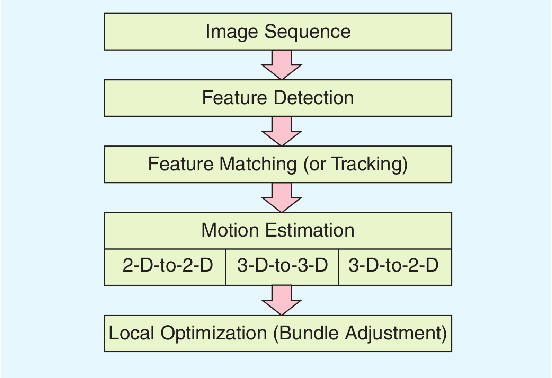
\includegraphics[width=0.5\textwidth]{Figures/DiagramaDeBlocosVO.png}
	\caption{Um diagrama de blocos mostrando os principais componentes de um componente de odometria visual \cite{yousif2015overview}.}
	\label{fig:Figures/dgblocoVO}
\end{figure}
\ \\
%% ------------------------------------------------------------------------- %%

\subsection{Visual Monocular}
\label{sec:visualmonocular}

De acordo com \cite{yousif2015overview}, no VO monocular, os pontos de recurso precisam ser observados em pelo menos três quadros diferentes (observe os recursos no primeiro quadro, re-observe e triangule em pontos 3D no segundo quadro e calcule a transformação no terceiro quadro, Armação). Uma questão importante no VO monocular é o problema de ambiguidade da escala. Ao contrário dos sistemas de visão estéreo em que a transformação (rotação e translação) entre os dois primeiros quadros da câmera pode ser obtida, a transformação entre os dois primeiros quadros consecutivos na visão monocular não é totalmente conhecida (a escala é desconhecida) e geralmente é definida como um valor predefinido . Em \cite{wirth2013visual}, esses problemas também são considerados e descritos. Segundo o autor, sistemas que usam apenas uma câmera precisam de movimento de translação para estimativa de movimento em 3D e todas as medições precisam ser dimensionadas por um fator desconhecido para estar em uma escala métrica.

O uso de uma câmera estéreo calibrada supera os dois problemas mencionados, pois as coordenadas 3D dos pontos correspondentes em um único par de imagens esquerda/direita podem ser calculadas por triangulação.

A Figura~\ref{fig:Figures/MonocularVOSystem} apresenta as poses relativas entre as câmeras que visualizam o mesmo ponto 3D são calculadas combinando os pontos correspondentes na imagem 2D. Se a localização 3D dos pontos for conhecida, pode ser usado um método 3D para 3D ou 3D para 2D. As poses globais são calculadas concatenando as transformações relativas em relação a um quadro de referência (pode ser definido como o quadro inicial) \cite{yousif2015overview}
\ \\
\begin{figure}[!htb]
	\centering	
	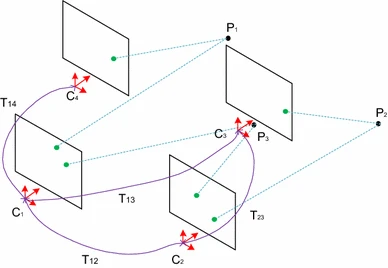
\includegraphics[width=0.6\textwidth]{Figures/MonocularVOSystem.png}
	\caption{Um exemplo de sistema VO monocular.}
	\label{fig:Figures/MonocularVOSystem}
\end{figure}
\ \\
As abordagens de VO foram apresentadas também para o domínio subaquático. Usando pipelines que incluem rastreamento de recursos e estimativa de movimento, esses sistemas são capazes de calcular transformações planares \cite{huang2017visual} ou seis graus de liberdade (DoF) \cite{wirth2013visual}, \cite{corke2007experiments} incrementais da pose da câmera. Medidas inerciais também podem ser incluídas para melhorar o desempenho \cite{creuze2017monocular}.

De acordo com \cite{bellavia2017selective}, os ambientes subaquáticos são tipicamente caracterizados por imagens não estruturadas, ruidosas e altamente texturizadas, com padrões repetitivos e más condições de iluminação local (efeitos de vinheta e outros artefatos). Consequentemente, os pontos-chave da imagem são difíceis de rastrear e corresponder corretamente debaixo d'água, mesmo se forem empregados detectores/descritores de recursos estáveis e robustos, como a transformação de recurso invariante em escala (SIFT) \cite{lowe2004distinctive}, os recursos robustos acelerados (SURF) \cite{bay2006surf} ou descritores de recursos com base nos momentos de Zernike \cite{eustice2008visually}, \cite{kim2009pose}.

A maioria das soluções subaquáticas propostas prefere configurações estéreo em vez de monoculares para melhorar a robustez e a precisão da saída, evitando problemas como os citados antes \cite{bellavia2017selective}, \cite{kim2013real}.
%% ------------------------------------------------------------------------- %%

\subsection{Visual Estéreo}
\label{sec:visualestereo}
\ \\
Usando o mesmo conceito do sistema visual humano, o sistema de visão estereoscópica ou estereoscópica emprega um conjunto de câmeras binoculares, como mostrado na Figura~\ref{fig:Figures/ImagensSimutaneas}. Segundo os autores em \cite{stivanello2008correspondencia}, um sistema estéreo pode extrair informações da cena observada recuperando dados de profundidade de um ponto no espaço a partir da distância relativa entre dois pontos. Essa diferença nas coordenadas dos pontos correspondentes às projeções é chamada disparidade.
\ \\
\begin{figure}[!htb]
	\centering	
	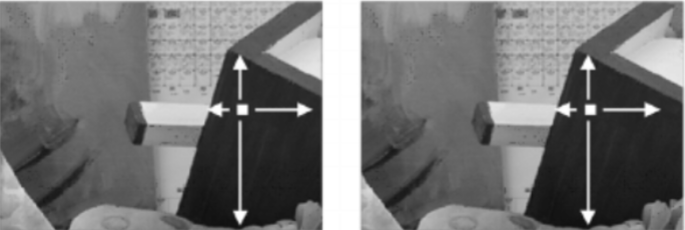
\includegraphics[width=0.7\textwidth]{Figures/ImagensSimutaneas.png}
	\caption{Imagem de duas lentes simultâneas \cite{stivanello2008correspondencia}.}
	\label{fig:Figures/ImagensSimutaneas}
\end{figure}
\ \\
A geometria necessária para fornecer a terceira dimensão é baseada no conceito de geometria epipolar, onde duas câmeras são apontadas para a mesma cena em duas posições distintas, resultando em várias conexões geométricas entre elas e, portanto, fornecendo os pontos 3D, epipolar. A geometria é apresentada com mais detalhes em \cite{bappy2012study}.

\begin{figure}[!htb]
	\centering	
	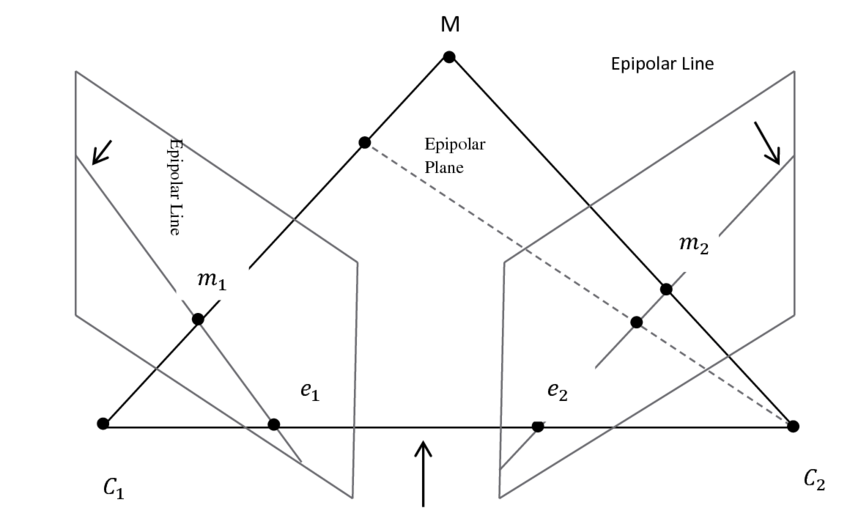
\includegraphics[width=0.5\textwidth]{Figures/EpipolarGeometry.png}
	\caption{Conceito de geometria epipolar \cite{bappy2012study}.}
	\label{fig:Figures/EpipolarGeometry}
\end{figure}
\ \\
A odometria visual (VO) é o processo de estimar o movimento de um veículo em movimento usando a entrada de vídeo de suas câmeras a bordo.

No VO estéreo, o movimento é estimado pela observação de recursos em dois quadros sucessivos (nas imagens direita e esquerda). Na Figura~\ref{fig:Figures/Clound3DPoints}, são mostrados quadros rastreados para formar uma nuvem de pontos 3D esparsos do ambiente e podem ser usados como base para a localização.
\ \\
\begin{figure}[!htb]
	\centering	
	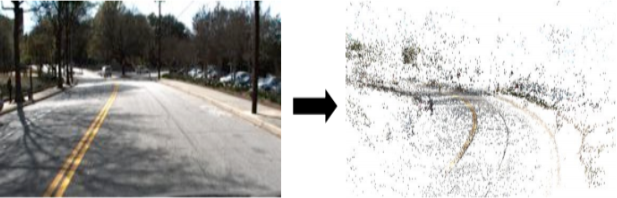
\includegraphics[width=0.8\textwidth]{Figures/Clound3DPoints.png}
	\caption{Os quadros rastreados formam uma nuvem de pontos 3D \cite{stivanello2008correspondencia}.}
	\label{fig:Figures/Clound3DPoints}
\end{figure}
\ \\
De acordo com os autores em \cite{stivanello2008correspondencia}, uma das principais vantagens da visão estéreo é que as imagens armazenam uma quantidade enorme de informações significativas, mesmo sem a necessidade de mover a câmera, além disso, fornecem alta precisão da localização, provando ser barata. solução em comparação com outros sensores de proximidade. Em \cite{zhou2017robust}, devido à certa linha de base entre as câmeras esquerda e direita, o problema de escala de ambiguidade é estabelecido e provado que não existe no VO estéreo. Além disso, o VO estéreo pode estimar o 6-Degree of Freedom (DOF) e o sensor do movimento do ego, o que não diz respeito ao tipo de ambiente em que o sistema trabalha. Atualmente, existem dois tipos de métodos de VO estéreo, 3D-3D e 3D-2D.

De acordo com \cite{yousif2015overview}, essa estimativa de movimento 3D-3D é realizada triangulando pontos de recurso 3D observados em uma sequência de imagens. A transformação entre os quadros da câmera é então estimada minimizando a distância euclidiana 3D entre os pontos 3D correspondentes.

Os autores também discutiram sobre o método de estimativa de movimento 3D-2D semelhante à abordagem anterior, mas aqui o erro de re-projeção 2D é minimizado para encontrar a transformação necessária. Novamente, o número mínimo de pontos requeridos varia com base no número de restrições no sistema.
Embora esses métodos de VO estéreo tenham se mostrado promissores, existem alguns problemas em relação à captura de imagens, gerando desvio de trajetória e valores discrepantes, como condições de iluminação, textura ao redor, presença de água, neve, desfoque de movimento, presença de sombras, semelhança visual, configuração degenerada e oclusões.

Com o objetivo de avaliar a melhor abordagem para estimativa de localização, a comparação de desempenho entre as abordagens de VO estéreo e VO monocular foi realizada em \cite{chen2015performance}. Figura~\ref{fig:Figures/DemoPerMonocular}, a trajetória no movimento de curvatura pode ser facilmente distinguida com o caminho de referência no modo monocular. O valor da distância percorrida é de 6,3\%, o principal motivo é que o resultado da correspondência monocular não é robusto o suficiente para fornecer uma boa estimativa de movimento quando o veículo está sob a dinâmica de viragem. Além disso, há um problema de ambiguidade de escala no resultado.

Portanto, o sistema VO estéreo tem desempenho mais estável que o sistema monocular, e a superioridade pode ser verificada através do experimento de tornar dinâmico em \cite{chen2015performance}.

Figura~\ref{fig:Figures/AnaliseOdometria}, é mostrada a comparação de desempenho entre o sistema de integração INS (Sistema de Navegação Inercial)/GNSS (Sistema Global de Navegação por Satélite), que é um dos mais usados na área de navegação, e a abordagem VO (Odometria Visual), respectivamente para sistemas monocular e estéreo. A taxa de amostragem mais alta tem melhor desempenho tanto na trajetória pura quanto na TD (Distância percorrida), tanto E (leste) (m) quanto N (norte) (m), quando o veículo passa por algumas áreas onde a qualidade do sinal GPS recebido é instável, o INS/GPS MEMS (Micro Sistemas Eletromecânicos) com o esquema fracamente acoplado gerará facilmente piores soluções de navegação \cite{chen2015performance}.
\ \\
\begin{figure}[!htb]
	\centering	
	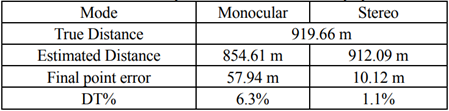
\includegraphics[width=0.6\textwidth]{Figures/AnaliseOdometria.png}
	\caption{A análise numérica de dois sistemas de odometria visual em que a comparação é curva é mostrada na Figura~\ref{fig:Figures/DemoPerMonocular} e na Figura~\ref{fig:Figures/DemoPerEstereo}
	\cite{chen2015performance}.}
	\label{fig:Figures/AnaliseOdometria}
\end{figure}
\ \\
\begin{figure}[!htb]
	\centering	
	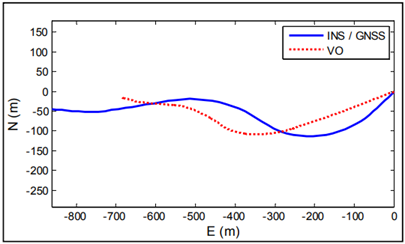
\includegraphics[width=0.6\textwidth]{Figures/DemoPerMonocular.png}
	\caption{Demonstração de VO monocular de desempenhos com mais distorção
	\cite{chen2015performance}.}
	\label{fig:Figures/DemoPerMonocular}
\end{figure}
\ \\
\begin{figure}[!htb]
	\centering	
	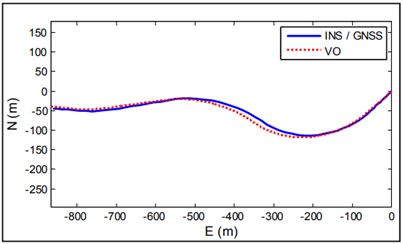
\includegraphics[width=0.6\textwidth]{Figures/DemoPerEstereo.png}
	\caption{VO estéreo, demonstrativa de desempenho mais estável \cite{chen2015performance}.}
	\label{fig:Figures/DemoPerEstereo}
\end{figure}
\ \\
%% ------------------------------------------------------------------------- %%

\section{Visual SLAM}
\label{sec:visualslam}

De acordo com \cite{yousif2015overview}, \cite{fraundorfer2011visual} SLAM é uma maneira de um robô se localizar em um ambiente desconhecido, enquanto constrói incrementalmente um mapa de seus arredores. O SLAM foi extensivamente estudado nas últimas décadas, resultando em muitas soluções diferentes usando sensores diferentes, incluindo sensores de sonar, sensores de infravermelho e scanners LASER. Recentemente, houve um interesse crescente no SLAM baseado em visual, também conhecido como V-SLAM, devido às informações visuais ricas disponíveis nos sensores de vídeo passivos de baixo custo em comparação aos scanners LASER.

De acordo com \cite{fraundorfer2011visual}, \cite{nister2004visual}, o objetivo do V-SLAM é obter uma estimativa global e consistente do caminho do robô. Isso implica manter um controle de um mapa do ambiente (mesmo no caso em que o mapa não é necessário per se) porque é necessário perceber quando o robô retorna a uma área visitada anteriormente, esse processo é conhecido como detecção de fechamento de loop. Quando um fechamento de loop é detectado, essas informações são usadas para reduzir a deriva no mapa e no caminho da câmera. De acordo com \cite{wirth2013visual}, os algoritmos para odometria visual - em oposição aos algoritmos SLAM completos - concentram-se em estimativas rápidas de movimento quadro a quadro, sem manter um grande histórico de fechamento de loop.

A ênfase está em medições precisas em altas frequências. Entender quando ocorre um fechamento de loop e integrar eficientemente essa nova restrição no mapa atual são dois dos principais problemas do V-SLAM. Uma das principais desvantagens da implementação das técnicas do V-SLAM depende do tempo de computação e utiliza recursos que, por sua vez, crescem significativamente para grandes ambientes \cite{nawaf2017towards}. Em \cite{strasdat2012visual} é apresentada uma pesquisa extensa considerando outros aspectos relacionados ao V-SLAM e aplicações similares.
%% ------------------------------------------------------------------------- %%


%\chapter{Revis\~ao da literatura especializada - Fundamenta\c{c}\~ao te\'orica do Tema 2}
%\label{chapter:tema2}

\chapter{O Projeto \rovname}
\label{chapter:contrucaorov}

Esta seção pode conter a construção do ROV.

\section{Desenvolvimento do Projeto}
\label{sec:desenvolvimentodoprojeto}

%% ------------------------------------------------------------------------- %%
\subsection{Softwares}
\label{sec:softwares}

texto texto texto texto texto texto texto texto texto texto
texto texto texto texto texto texto texto texto texto texto
texto texto texto texto texto texto texto texto texto texto

\subsubsection{Ubuntu Linux 16.04}
\label{sec:ubuntulinux}

De acordo com \cite{whatisUbuntu}, O Ubuntu é um sistema operacional Linux completo, disponível gratuitamente (Open-Source) com suporte comunitário e profissional. O Projeto Ubuntu é patrocinado pela \cite{canonical}. A Canonical não cobrará taxas de licença pelo Ubuntu, agora ou em qualquer estágio no futuro. O modelo de negócios da Canonical é fornecer suporte técnico e serviços profissionais relacionados ao Ubuntu.

\subsubsection{ROS e Gazebo (Ambiente de Simulação)}
\label{sec:rosegazebo}

De acordo com \cite{ROSIntroduction}, O ROS é um sistema meta-operacional de código aberto. Fornece os serviços como abstração de hardware, controle de dispositivo de baixo nível, comumente usado funcionalidade, passagem de mensagens entre processos e pacote gestão.

De acordo com \cite{gazebo}, Gazebo É o simulador de física do mundo real, oferecendo a capacidade de simular com precisão e eficiência populações de robôs em ambientes internos e externos complexos sendo gratuito com uma comunidade ativa.

\subsubsection{Gephi (Pacote de software de análise e visualização de rede)}
\label{sec:gephi}

texto texto texto texto texto texto texto texto texto texto
texto texto texto texto texto texto texto texto texto texto
texto texto texto texto texto texto texto texto texto texto

\subsubsection{Draw.io (Aplicação de diagramação gráfica online)}
\label{sec:drawio}

texto texto texto texto texto texto texto texto texto texto
texto texto texto texto texto texto texto texto texto texto
texto texto texto texto texto texto texto texto texto texto

\subsubsection{Solidworks (Software CAD 3D (Design Assistido por Computador))}
\label{sec:solidwoks}

texto texto texto texto texto texto texto texto texto texto
texto texto texto texto texto texto texto texto texto texto
texto texto texto texto texto texto texto texto texto texto

\subsubsection{Cura (Software fatiador e servidor para impressora 3D)}
\label{sec:cura}

texto texto texto texto texto texto texto texto texto texto
texto texto texto texto texto texto texto texto texto texto
texto texto texto texto texto texto texto texto texto texto
%% ------------------------------------------------------------------------- %%

\subsection{Desenho Técnico}
\label{sec:desenhotecnico}

Apresentação da vista do desenho técnico do \rovname \space desenvolvido e renderizado no SolidWorks, como é mostrado nas figuras Figura~\ref{fig:Projvistatotal}, Figura~\ref{fig:Projvistafrnotal}, Figura~\ref{fig:Projvistainferior} e Figura~\ref{fig:Projvistasuperior}, vista geral, vista frontal, vista inferior e superior respectivamente.

\begin{figure}[!htb]
	\centering	
	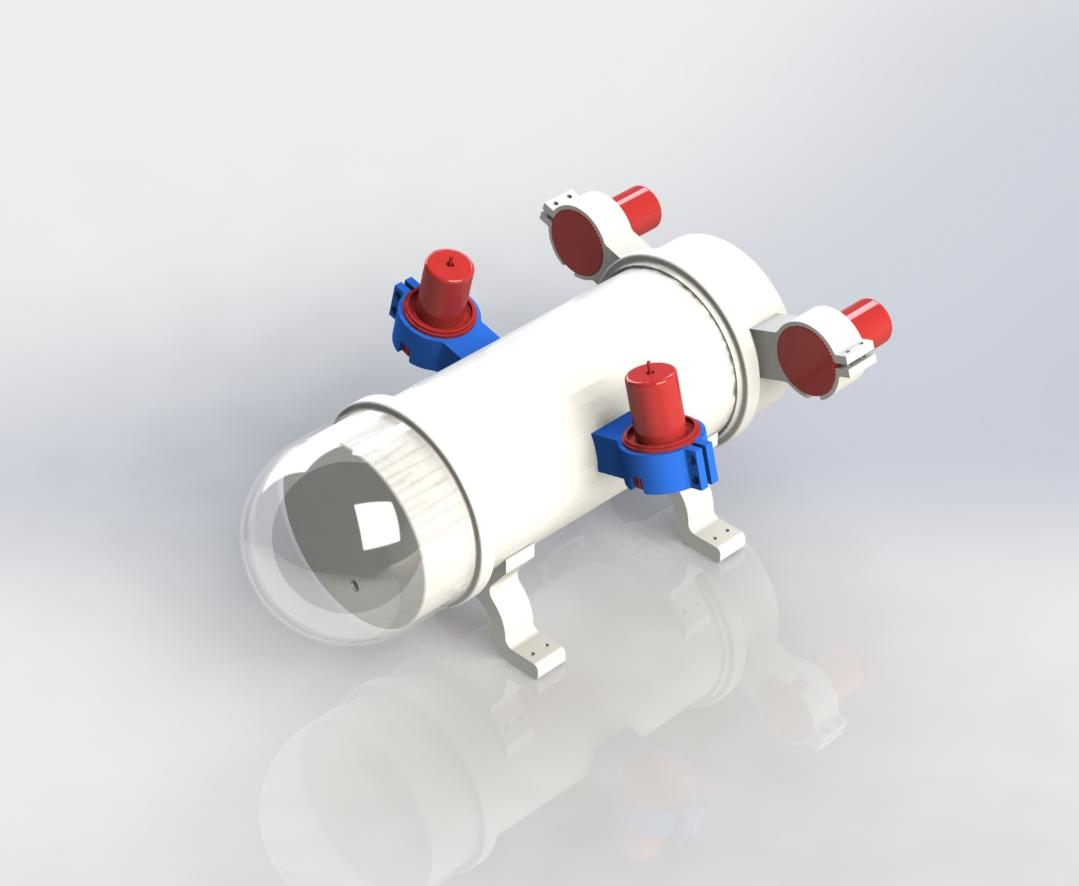
\includegraphics[width=0.5\textwidth]{Figures/Rov/Proj_vista_total.jpeg}
	\caption{Vista Total, Fonte: Elaborada pelo autor\the\year}
	\label{fig:Projvistatotal}
\end{figure}

\begin{figure}[!htb]
	\centering	
	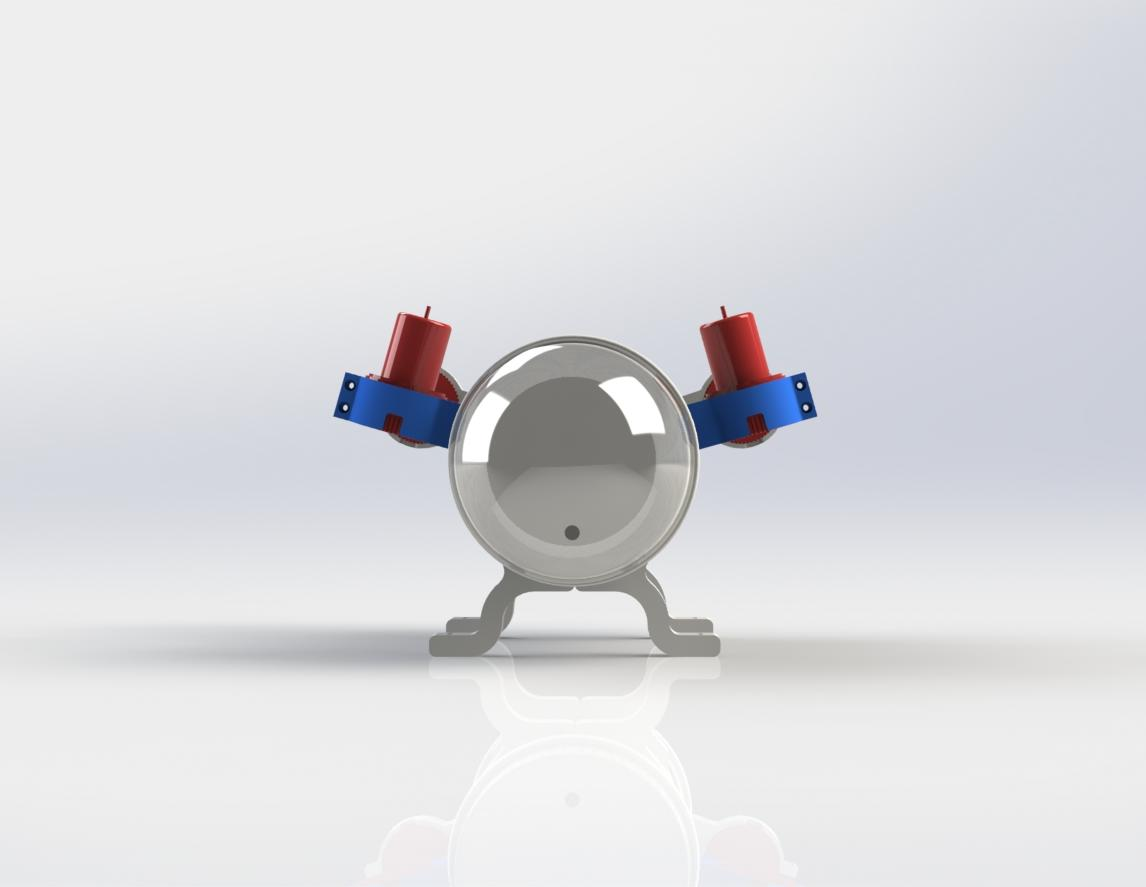
\includegraphics[width=0.5\textwidth]{Figures/Rov/Proj_vista_frontal.jpeg}
	\caption{Vista Frontal, Fonte: Elaborada pelo autor\the\year}
	\label{fig:Projvistafrnotal}
\end{figure}

\begin{figure}[!htb]
	\centering	
	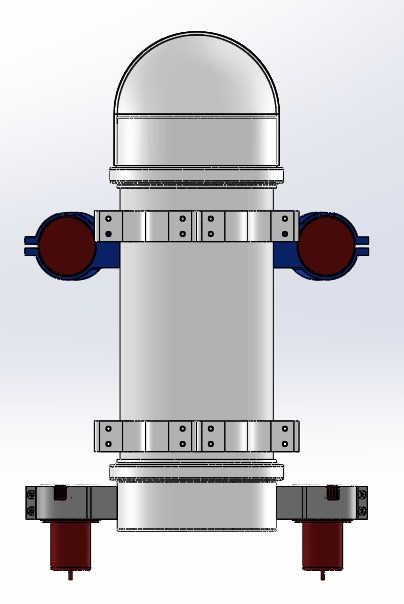
\includegraphics[angle=90,width=0.5\textwidth]{Figures/Rov/Proj_vista_inferior.jpeg}
	\caption{Vista Inferior, Fonte: Elaborada pelo autor\the\year}
	\label{fig:Projvistainferior}
\end{figure}

\begin{figure}[!htb]
	\centering	
	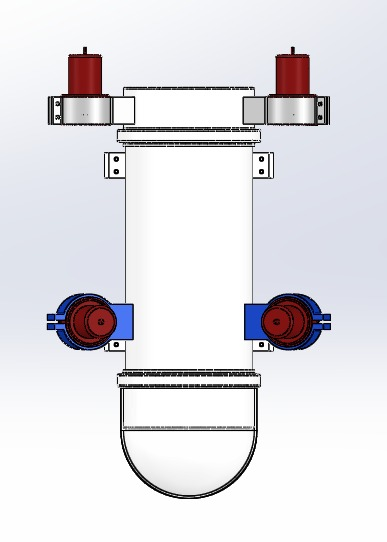
\includegraphics[angle=90,width=0.5\textwidth]{Figures/Rov/Proj_vista_superior.jpeg}
	\caption{Vista Superior, Fonte: Elaborada pelo autor\the\year}
	\label{fig:Projvistasuperior}
\end{figure}

%% ------------------------------------------------------------------------- %%

\subsection{Estrutura (Chassi)}
\label{sec:estruturachassi}

texto texto texto texto texto texto texto
texto texto texto texto texto texto texto
texto texto texto texto texto texto texto

Materiais utilizados para a construção.

\begin{itemize}
    \item 1 - Tubo PVC 150mm;
    \item 4 - Bomba De Porão Seaflo 1100gph - 4164lph 12v;
    \item 2 - Tampas PVC 150mm com borracha;
    \item 4 - Suportes impressos em PLA 3d;
    \item 4 - Hélices de plástico;
    \item 1 - Arduíno Mega 2560;
    \item 2 - Ponte H Monster Motor Shield VNH2SP30 30a 2 Motor;
    \item 1 - Cúpula Acrílica Hemisférica;
    \item 40 - Parafusos de aço inox com porca;
    \item 15 - Metros de fios awg22;
\end{itemize}

\begin{figure}[!htb]
	\centering	
	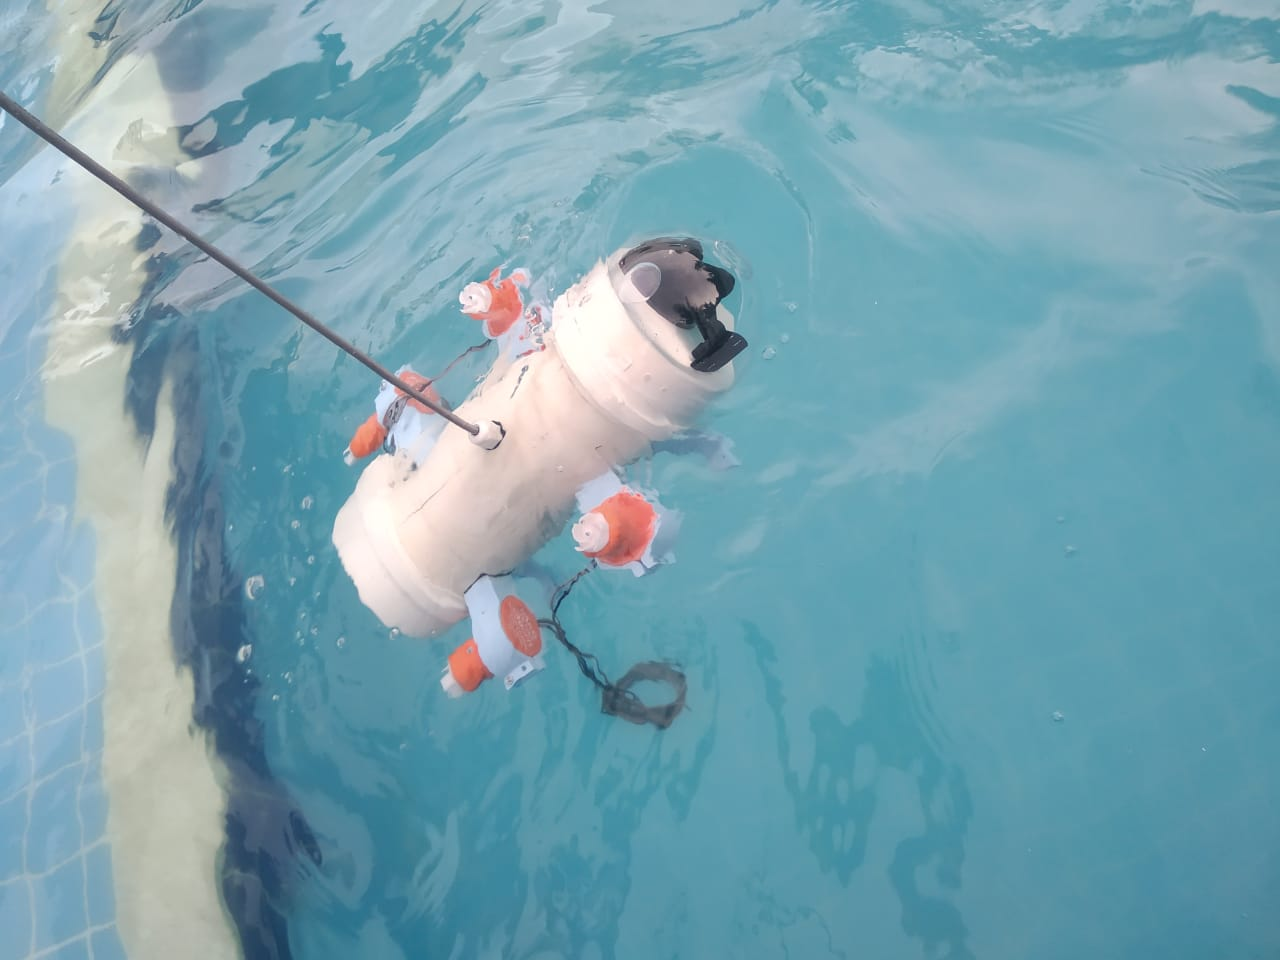
\includegraphics[width=0.5\textwidth]{Figures/Rov/Estrutura_ROV.jpeg}
	\caption{Vista Superior, Fonte: Elaborada pelo autor\the\year}
	\label{fig:estruturarov}
\end{figure}
%% ------------------------------------------------------------------------- %%

\subsection{Motores de Tração}
\label{sec:motoresdetracao}

De acordo com \cite{bombadeporao}, As bombas de esgoto não-automáticas 1100GPH da SEAFLO oferecem evacuação de água ativada por um painel ou interruptor de bóia alem de Incluir proteção de bloqueio anti-ar e vedações herméticas exclusivas, fiação de bloco de grau marítimo. Disponível para tensão 12 e 24 tensão. O modelo 1100GPH 12V, atende as especificações do projeto devido ao seu alto torque e selagem hermética, possibilitando uma submersão de até 20 pés (6,096) metros.

Principais Características:

\begin{itemize}
    \item 2 anos de garantia
    \item Atende ou excede os padrões RoHS, SGS e ISO
    \item Operação tradicional por interruptor ou interruptor de bóia
    \item Totalmente submersível
    \item Base do filtro de encaixe para fácil manutenção
    \item Bomba e interruptor são produtos independentes
    \item Motores eficientes e de longa vida útil selados
    \item Funciona a seco, capaz de cargas de trabalho normais
    \item Operação silenciosa
    \item limites de temperatura de $110\,^{\circ}\mathrm{F}$ ($43\,^{\circ}\mathrm{C}$)
    \item eixo de aço inoxidável
    \item Proteção anti-Airlock
    \item Selos herméticos exclusivos
    \item Fiação bloqueada de grau marítimo
\end{itemize}

\begin{figure}[!htb]
	\centering
	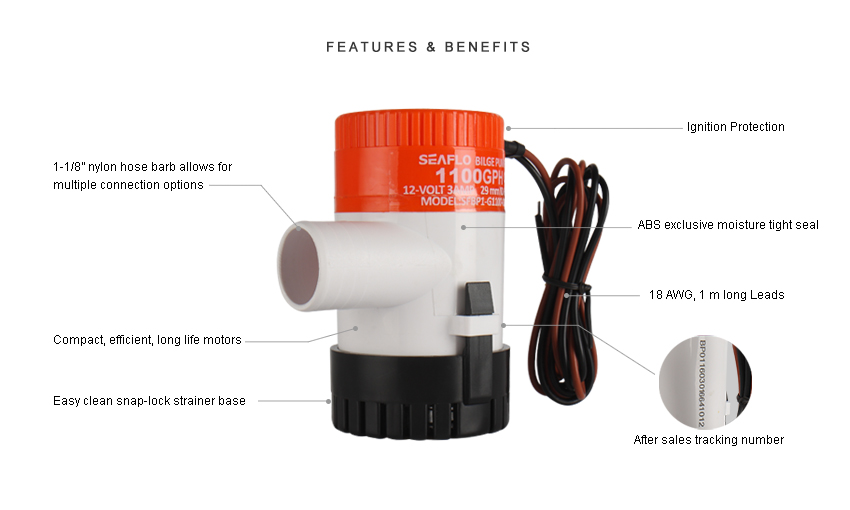
\includegraphics[width=0.8\textwidth]{Figures/Rov/Bomba_porao-Seaflo.jpg}
	\caption{Vista Superior, \cite{bombadeporao}}
	\label{fig:bombaporao}
\end{figure}
%% ------------------------------------------------------------------------- %%

\subsection{Cabos e Conexões}
\label{sec:caboseconexoes}

%% ------------------------------------------------------------------------- %%

\subsection{Sensores}
\label{sec:sensores}
%% ------------------------------------------------------------------------- %%

\subsection{Microcontroladores}
\label{sec:microcontroladores}

O sistema embarcado utilizado para controlar as entradas e saídas de comandos lógicos do \rovname.

\subsubsection{Arduino}
\label{sec:arduino}
(+ texto)

\subsubsection{Raspberry Pi}
\label{sec:raspberrypi}
(+ texto)
%% ------------------------------------------------------------------------- %%

\subsection{Ponte-H}
\label{sec:ponteh}

De acordo com \cite{monstermotorshield}, O VNH2SP30 é um driver de motor de ponte que incorpora um driver monolítico duplo alto e dois interruptores laterais baixos, os pinos do sensor de corrente (CS) produzirão aproximadamente 0,13 volts por amp de corrente de saída. Sendo uma ótima escolha já que o mesmo é capaz de controlar até dois motores com corrente de pico de 30A, controlando o sentido de rotação e velocidade do motor.

Principais Características:

\begin{itemize}
	\item Tensão máxima: 30V;
    \item Máxima corrente: 30 A;
    \item Corrente nominal de operação: 14 A;
    \item Medição de corrente disponível para o Arduino nos pinos analógicos;
    \item MOSFET sobre resistência: 19 m$\Omega$;
    \item Frequência PWM máxima: 20 kHz;
    \item Proteção térmica;
    \item Proteção contra sobretensão e subtensão;
\end{itemize}

\begin{figure}[!htb]
	\centering	
	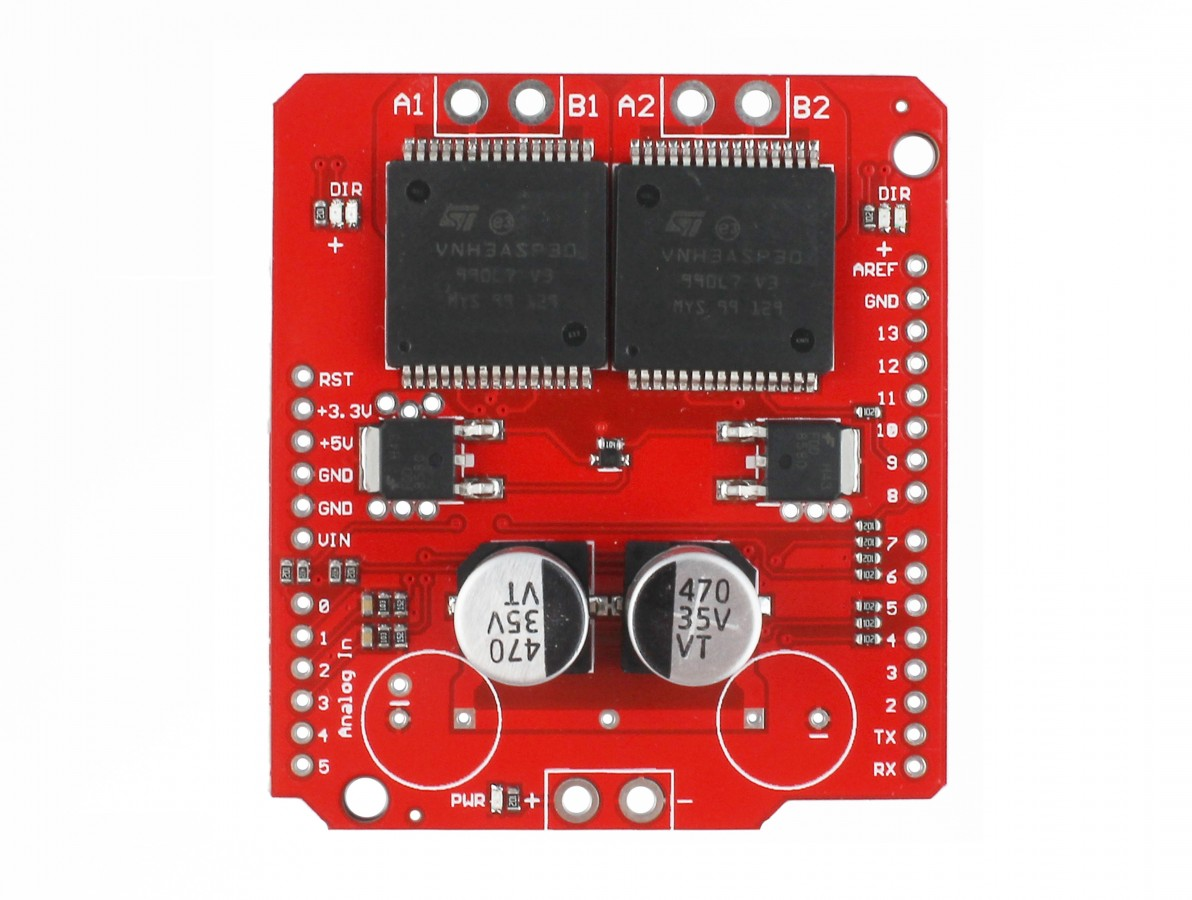
\includegraphics[width=0.5\textwidth]{Figures/Rov/Monster_motor_shield.jpg}
	\caption{Vista Superior Monster Motor Shield \cite{monstermotorshield}}
	\label{fig:monstermotorshield}
\end{figure}
%% ------------------------------------------------------------------------- %%

\subsection{Fonte de Alimentação}
\label{sec:fontedealimentacao}
%% ------------------------------------------------------------------------- %%

\subsection{Painel de Controle}
\label{sec:paineldecontrole}
%% ------------------------------------------------------------------------- %%

\chapter{Trabalho experimental e desenvolvimento da pesquisa}
\label{chapter:trabalhoexperimental}



\section{Modelo proposto}
\label{section:titulo41}


\section{An\'alise experimental/Simula\c{c}\~oes e cen\'arios}
\label{section:titulo42}


\section{Resultados}
\label{section:titulo43}


\section{Discuss\~ao}
\label{section:titulo4N}

\chapter{Título do capítulo}\label{chapter:outro}

\textcolor{red}{As organizações atuam em um ...}
%
\chapter{Scenario Definitions and Network Analysis}\label{chpdata}

This chapter illustrates the use of our model to represent a real world population,
summarises the model's options and examines the properties of the underlying small world
network representation for a variety of scenarios. It highlights and contrasts the
model's strengths and weaknesses as compared with the original small world model
\cite{Watts1998} and traditionally used social network models.


\section{Scenarios}

The data used to define the population scenarios for analysis and validation of this
model comes from Brazil. A national study conducted in 2000, evaluated the sexual
behaviour of the Brazilian population and perception of HIV/AIDS \cite{msbrasil2000}. The
study consisted of a face to face interview of 3,600 males and females ageing between 16
and 65 years and living in urban areas of 169 micro regions of Brazil. The micro regions
were defined by the Brazilian 1996 census. The urban population in this age range was
77,018,813 people and the sample region represents a population of 59,872,819 people,
corresponding to 77.7\% of this population.

A similar study was conducted in 2003 by the Brazilian National STD/AIDS programme to
investigate the behaviour of the sexually active population in the past six months, 14
years of age and above \cite{msibope2003}. This second study focused only on sexual
behaviour and safe sex practice of the population; 1,298 face to face interviews were
conducted nationwide.

A further follow-up survey entitled the \emph{Knowledge, Attitudes and Practices of the
Brazilian Population aged between 15 and 54 years} \cite{Szwarcwald2004} expanding on the
first and second was completed in 2004. A total of 6,000 individuals were interviewed,
the sample was stratified according to geographic region (macro-region): 900 interviews
were conducted in the North, South and Centre-West regions, 1,100 in the Northeast region
and 2,200 in the Southeast. In each of the major regions, the sample was carried out in
multiple stages: States; census sectors; and households. The sectors within each of the
States were selected by systematic sampling, with probability proportional to size.

\newpage
The data from the second and the third studies is also available and was used to adjust
the parameters fitted to the first study due to observed sexual behavioural changes
during the four years gap. For clarity the data is not presented here but in Appendix
\ref{chpfitting}. The way that parameters were estimated and the model was fitted is also
described in detail in Appendix \ref{chpfitting}. The following two scenarios will be
used to verify and validate the model as a small world network, illustrate its use to
represent a real world population and the flexibility of the model implementation.

\subsection{Single Group}\label{scenariosingle}

Table \ref{singlegroup} defines a single group representation of the population; this
scenario will be used to illustrate the properties of the social network, the effects of
sexual behavioural change and social interactions on the dynamics of the sexual
transmission of HIV in a small world network.

\begin{longtable}[c]{|p{9cm}|c|}
\caption{Single group scenario definition}\label{singlegroup}\\ \hline
\bfseries Parameters and probability distributions & \bfseries Value (months) \\\hline\hline
\endfirsthead

\multicolumn{2}{c} {{\tablename} \thetable{} -- Continued} \\\hline
\bfseries Parameters and probability distributions & \bfseries Value (months) \\\hline\hline
\endhead
\multicolumn{2}{r}{\emph{Continued on next page}}
\endfoot
\endlastfoot

Population size (\emph{n})      & 3,324  \\\hline
Age distribution                & Weibull(181.47, 267.95, 1.46) \\\hline
Life expectancy                 & 840 (70 years) \\\hline
Proportion of females           & 0.55  \\\hline
Proportion of males             & 0.45  \\\hline
Proportion of homosexual males  & 0.05  \\\hline\hline
HIV prevalence                  & 0.007 \\\hline
HIV lead-time distribution                                    & Weibull(0.13, 47.78, 1.36) \\\hline
HIV testing rate                                              & 0.28 \\\hline\hline
Maximum number of concurrent partnerships                     & 5    \\\hline
Probability of concurrent partnership                         & 0.11 \\\hline
Probability of a casual partnership                           & 0.18 \\\hline
Probability of looking for a sexual partner at any time       & 0.82 \\\hline
Probability of searching own group first for a casual partner & 1    \\\hline\hline
Duration of stable partnerships                                                   & Weibull(141.36, 1.10) \\\hline
Time between stable partnerships                                                  & Gamma(20.20, 1.06) \\\hline
Rate of sexual intercourse for stable partnership per unit of time                & Gamma(4.83, 1.41) \\\hline
Probability of safe sex practice during sexual intercourse for stable partnership & 0.18 \\\hline\hline
Duration of casual  partnerships                                                  & InvNormal(-2.44, 14.49, 49.60) \\\hline
Rate of sexual intercourse for casual partnership per unit of time                & Gamma(5.02, 1.5) \\\hline
Probability of safe sex practice during sexual intercourse for casual partnership & 0.42 \\\hline
\end{longtable}

\subsection{Multiple Groups}\label{scenariomulti}

Table \ref{multigroup} defines a multi group representation of the Scenario
\ref{scenariosingle} population. It is important to notice the overlapping of the group
definition for \emph{under 25} and \emph{married} groups. In this case, being married has
higher priority over age, therefore less than 25 years of age and married individuals are
classified as part of the married sub group. This scenario will be used to evaluate the
effects of inter core group interactions on the dynamics of the sexual transmission of
HIV in a small world network. For simplicity the initial HIV prevalence will be kept
unchanged.

\begin{landscape}
\begin{longtable}[c]{|p{8.1cm}|c|c|c|}
\caption{Multi group scenario definition}\\ \hline
\bfseries \multirow{2}{8.1cm}{Parameters and probability distributions} & \multicolumn{3}{|c|}{\bfseries Groups Definition (months)} \\
\cline{2-4} & \bfseries Married & \bfseries Under 25 & \bfseries Others \\\hline\hline
\endfirsthead

\multicolumn{4}{c} {{\tablename} \thetable{} -- Continued} \\\hline
\bfseries \multirow{2}{8.1cm}{Parameters and probability distributions} & \multicolumn{3}{|c|}{\bfseries Groups Definition (months)} \\
\cline{2-4} & \bfseries Married & \bfseries Under 25 & \bfseries Others \\\hline\hline
\endhead

\multicolumn{4}{r}{\emph{Continued on next page}}
\endfoot
\endlastfoot
\label{multigroup}
Population size (\emph{n})      & 1422 & 794 & 1108 \\\hline
Age distribution                & \small{Weibull(182.3, 336.28, 2.29)}& \small{LogNormal(143.95, 95.05, 36.99)} & \small{InvNormal(242.15, 246.94, 621.89)}\\\hline
Life expectancy (70 years)      & 840 & 840 & 840 \\\hline
Proportion of females           & 50\%   & 45.7\% & 62.4\% \\\hline
Proportion of males             & 50\%   & 54.3\% & 37.6\%\\\hline
Proportion of homosexual males  & 5\%    & 5\%    & 5\%  \\\hline\hline
HIV prevalence                  & 0.007   & 0.007   & 0.007 \\\hline
HIV lead-time distribution      & Weibull(64.26, 1.63) & Weibull(71.79, 1.61) & Weibull(64.26, 1.63) \\\hline
HIV testing rate                & 16.34\% & 11.71\% & 18.29\% \\\hline\hline
Maximum number of concurrent partnerships                     & 5 & 5 & 5 \\\hline
Probability of concurrent partnership                         & 0.06 & 0.21 & 0.14 \\\hline
Probability of a casual partnership                           & 0.06 & 0.40 & 0.27 \\\hline
Probability of looking for a sexual partner at any time       & 1 & 0.78 & 0.64 \\\hline
Probability of searching own group first for a casual partner & 0.4 & 0.8 & 0.7 \\\hline\hline
Duration of stable partnerships                                                   & Weibull(198.19, 1.55) & LogNormal(29.77, 37.2) & Weibull(89.74, 1.01) \\\hline
Time between stable partnerships                                                  & Gamma(20.16, 1.07) & Weibull(14.89, 1.10) & Gamma(24.38, 1.03) \\\hline
Rate of sexual intercourse for stable partnership per unit of time                & Gamma(4.71, 1.51)  & Gamma(6.5, 1.06)     & Gamma(5.09, 1.34) \\\hline
Probability of safe sex practice during sexual intercourse for stable partnership & 0.11 & 0.47 & 0.21 \\\hline\hline
Duration of casual  partnerships                                                  & Gamma(8.84, 1.14) & Gamma(5.25, 1.03) & LogNormal(9.16, 14.61) \\\hline
Rate of sexual intercourse for casual partnership per unit of time                & Gamma(5.01, 1.58) & Gamma(7.1, 1.1) & Gamma(5.31, 1.39)  \\\hline
Probability of safe sex practice during sexual intercourse for casual partnership & 0.12 & 0.55 & 0.42 \\\hline
\end{longtable}

\begin{longtable}[c]{|c|c|c|c|}
\caption{Multi group default mixing matrix}\\ \hline
\label{multimixmat}
$\Rightarrow \oslash \Rightarrow $ & Married & Under 25 & Others \\\hline
& & & \\
Married  & x       & 0.5      & 0.5    \\
& & & \\\hline
& & & \\
Under 25 & 0.5     & x        & 0.5    \\
& & & \\\hline
& & & \\
Others   & 0.5     & 0.5      & x      \\
& & & \\\hline
\end{longtable}

\end{landscape}

The population mixing matrix defined in Table \ref{multimixmat} is given as default and
assumes that the flow of people between any two groups is the same on both directions.
However this is not the case for most real world situations and one should tune these
parameters in order to give a more realistic representation of the direction of external
interactions between different core groups' populations.

\subsection{HIV Infection}

The variables required by the model to represent the transmissibility and natural history
of the STD infection have been specified in section \ref{stddefsection}. Table
\ref{hivdefinition} defines the characteristics of the HIV transmission and progress from
infection to AIDS death without HAART intervention.

\begin{longtable}[c]{|p{8cm}|c|c|}
\caption{Transmissibility and natural history of HIV infection}\\\hline
\label{hivdefinition}
\textbf{Probability of HIV Transmission}     & \textbf{Value} & \textbf{References}  \\\hline
Female to Male                               & 0.002 &  \cite{Donovan2000,Royce1997} \\\hline
Male to Female                               & 0.003 &  \cite{Donovan2000,Royce1997} \\\hline
Male to Male                                 & 0.010 &  \cite{Donovan2000,Royce1997} \\\hline
\multicolumn{3}{|l|}{\textbf{Infection Characteristics}}\\\hline
Lifelong infection?                          & Yes   &  \\\hline
Duration of infection                        & N/A   &  \\\hline
Allow reinfection?                           & No    &  \\\hline
Mortality rate                               & 98\%  & \cite{UNAIDSRG2002} \\\hline
\multicolumn{3}{|l|}{\textbf{Natural History of HIV infection}}\\\hline
Progression from HIV infection to AIDS death & Weibull (126.12, 2.38) & \cite{UNAIDSRG2002} \\\hline
\end{longtable}


\subsection{Global Settings}\label{globalsettings}

The model's global configuration guides how the simulation behaves during run-time as
well as defines the constraints for calculation of the network global efficiency, length
of simulation warm-up, distribution of the initially infected individuals within the
population and the network structure. Table \ref{hivacsimconfig} defines the default global settings that
will be used throughout the model evaluation and validation. Changes to this global
configuration will be explicitly stated when they are required for the demonstration of a
specific property or condition.

\begin{longtable}[c]{|p{10cm}|c|c|}
\caption{HIVacSim global configuration and network structure definition}\\\hline
\label{hivacsimconfig}
\textbf{Simulation Properties}     & \textbf{Value} & \textbf{References}  \\\hline
Clock                                       & Month & \ref{hivacsim} \\\hline
Duration (12 years)                         & 144   & \ref{hivacsim} \\\hline
Replications (Runs)                         & 100   & \ref{hivacsim} \\\hline
\multicolumn{3}{|l|}{\textbf{Global Efficiency Calculation}}\\\hline
Switch algorithm at small world probability \emph{p} value & 0.13      & \ref{netinfo}\\\hline
Maximum network size for numerical calculation      & 500       & \ref{netinfo}\\\hline
Size of the geodesic sample for estimation          & 400       & \ref{netinfo}\\\hline
\multicolumn{3}{|l|}{\textbf{Warm-up \ref{warmup} and Initial Infection}}\\\hline
Duration (2 years)                                  & 24     & Table \ref{warmupconfig} \\\hline
Minimum number of concurrent partnerships           & 2      & Table \ref{warmupconfig} \\\hline
Probability of concurrent partnership               & 0.5    & Table \ref{warmupconfig} \\\hline
Distribution of the initial infection               & Clustered & \ref{initinfdist}\\\hline
\multicolumn{3}{|l|}{\textbf{Network Structure}}\\\hline
Maximum size of the acquaintances list              & 50     & \ref{listsize}\\\hline
$\beta$ (maximum number of trials)                  & 1      & \ref{searchrel}\\\hline
Degrees of separation                               & 3      & \ref{searchrel}\\\hline
Expected number of people in one's neighbourhood    & 50     & \ref{structure}\\\hline
Radius of the real world (earth)                    & 6378   & \ref{structure}\\\hline
Network topology                                    & Sphere & \ref{structure}\\\hline
\end{longtable}

The network structure settings are defined at group level and as such they may assume
different values according with the size of each group's population. The values provided
in Table \ref{hivacsimconfig} for size of the acquaintances list and neighbourhood are
used for solving Equations \ref{egnofriends} and \ref{solvedistance} respectively within
each group definition. The maximum number of trials is also dependent on the population
size and therefore will have a similar effect on the searching for relationships
(\ref{searchrel}, b).

\section{Small World Network Properties}\label{swnproperties}

The characteristics and measurements of small world networks are described in Section
\ref{swnetworks}. This section evaluates the strengths to which the HIVacSim model
conforms to the general theory of small world networks. Scenario \ref{scenariosingle}
will be used for verification and validation of the small world model in this and the
next chapter unless specified otherwise. 15 replications of each experiment are used
throughout this exercise to produce the plots, error bars and to define confidence
limits.

The original small world model of Watts and Strogatz \cite{Watts1998} can be quantified
by two simple statistics: the clustering coefficient \emph{C} for measuring local density
and the mean geodesic length \emph{L} for measuring the global separation. A small world
network is defined as a broad region between regularity and randomness in which the
network is highly clustered and has a short path length. As discussed in Sections
\ref{smgraphs} and \ref{geodesic}, the original formulation of the mean geodesic length
by Watts and Strogatz \cite{Watts1998} is valid only for fully connected networks. This
is not always the case in the real world where not everyone has friends or is involved in
a sexual partnership all the time.

Figure \ref{connected} shows the frequency of fully connected network occurrences found
experimentally in this model as a function of the network randomness parameter \emph{p}
(\emph{x axis has multiple scales}). This clearly illustrates the limitation of the
original small world model formulation and supports the adoption of a more consistent and
meaningful notation (\ref{netefficiency}) to quantify the characteristics of a small
world network.
\begin{figure}[h]
\includegraphics[width=\textwidth]{connected}
\caption{Frequency of fully connected sexual network occurrences} \label{connected}
\end{figure}

Figure \ref{originalswn} gives the small world network characteristics \emph{L} and
\emph{C} evaluated according to the original formulation of Watts and Strogatz
\cite{Watts1998}. Note that the \emph{L} values have been calculated only for the
occurrences of a fully connected network. Nevertheless the small world effect is clearly
visible. At just a small amount of randomness $(p \sim 0.1)$, \emph{L} has almost reached
its minimum value, yet \emph{C} is about half of its maximum value.
\begin{figure}[ht]
\begin{center}
\includegraphics{originalswn}
\caption{Characteristics of a small world network} \label{originalswn}
\end{center}
\end{figure}

Another global measure depending upon full network connectivity is the diameter, defined
as the length of the longest geodesic (\ref{geodesic}). This measure has a close relation
with the mean geodesic length and therefore can be evaluated only for fully connected
networks. Figure \ref{diameter} shows the small world effect on network diameter.
\begin{figure}[!h]
\includegraphics{diameter}
\caption{Small world effect on network diameter} \label{diameter}
\end{figure}

\subsection{Network Efficiency}\label{netefficiency}

The concept of efficiency on small world networks has been introduced by Latora and
Marchiori \cite{Latora2001} for measuring the global and local efficiency of a network
(\ref{smnefficiency}); these measures are denoted by $E_g$ and $E_l$ respectively. From
this perspective a small world network can be rephrased as a network with high global and
high local efficiency, therefore exchanging information very efficiently both on a global
and on a local scale. Figure \ref{efficiency} shows the HIVacSim model's efficiency.
These values compare well with those provided by Latora and Marchiori \cite{Latora2001},
and therefore we concluded that the HIVacSim network model indeed represents a small
world network.
\begin{figure}[h]
\includegraphics[width=\textwidth]{efficiency}
\caption{HIVacSim model's global and local efficiency} \label{efficiency}
\end{figure}

The short paths represented by the global efficiency, provide high-speed communication
channels between distant parts of the network, thereby facilitating any dynamical process
that requires global coordination, transmission of information or propagation of
infectious disease. The local efficiency provides short distance communication, enabling
high-speed propagation of information or disease through local clusters within the
population.

The network efficiency has a good agreement with the original small world model
formulation due to Watts and Strogatz \cite{Watts1998} by reporting a normalised
$1/E_g(p)$ and $E_l(p)$ as shown in Figure \ref{efficiencyswn}.
\begin{figure}[h]
\begin{center}
\includegraphics{efficiencyswn}
\caption{Network efficiency as the original small world characteristics}
\label{efficiencyswn}
\end{center}
\end{figure}

Figure \ref{efficiencyswn} compares well with Figure \ref{originalswn}, produced using
the original formulation of the small world characteristics. The small discrepancies
between global efficiency and \emph{L} can be attributed to the fact that the values for
\emph{L} in Figure \ref{originalswn} have been calculated using only a fraction of the
data produced by the experiment due to its network connectivity requirement, which is not
the case for global efficiency.


\subsection{Clustering Coefficient}\label{swnclustering}

The small world clustering coefficient \emph{C} defined in Section \ref{clusteringcoef},
measures the overlapping of acquaintances within the population. This measure can be
calculated numerically for the fully connected regular (\ref{latticegraphs}), the random
(\ref{randomgraph}) and the original small world network models (\ref{clusteringcoef}).
However for disconnected networks there is no deterministic formulation and therefore
this quantity has been evaluated through Monte Carlo simulation. Figure \ref{clustering}
compares the clustering coefficient of our small world model with results obtained by
deterministic evaluation of equivalent regular and random networks.
\begin{figure}[ht]
\includegraphics[width=\textwidth]{clustering}
\caption{Small world clustering coefficient} \label{clustering}
\end{figure}

As shown in Figure \ref{connected}, regular networks are less likely to be fully
connected due to the lack of concurrency and absence of long distance connectivity among
individuals within the population. This behaviour has a direct impact on the clustering
coefficient of the small world network as shown in Figure \ref{efficiencyswn}. However
real world networks, and in particular sexual networks, rarely fall in this category as
being regular and fully connected at the same time. Therefore we conclude that the
clustering coefficient of our small world network model approaches both extremities of
the theoretical spectrum for regularity and randomness with good accuracy and precision,
so it is consistent with the general definition of the small world network theory.


\subsection{Degree Distribution}

The study of degrees has received enormous attention in social networks and as a
consequence, it is one of the most popular terms in the sociology literature. It refers
to the number of social connections that one possesses, the number of partners at a point
in time and so on. From a small world perspective, the degree distribution quantifies the
size of the lists of acquaintances, the popularity of individuals within the network.
Figure \ref{degreeavg} shows the small world effects on the average degree of the
individuals within our model, a non-linear relation between randomness and average degree
can be observed.
\begin{figure}[h]
\includegraphics{degreeavg}
\caption{Small world effect on the average degree distribution} \label{degreeavg}
\end{figure}

Application of degrees is as common in graph theory as it is in social networks. It forms
the basis of the network \emph{centrality}, a measure of the varying importance of the
individuals in a network according to some predefined criterion, a coefficient of the
popularity of an actor, also known as degree centrality (\ref{netcentrality}). Degrees
were also the basis of the reverse small world experiment \cite{Killworth1978}.

The degree distributions of the original small world models have been defined through a
set of equations in Section \ref{swndegreedist}. However, they do not match most real
world networks very well since this was not a goal of the original model in the first
place. We provide empirical results showing the small world effect on degree distribution
of individuals within our model.

Figures \ref{degreepdf} and \ref{degreecdf} give the degree probability density function
(PDF) and cumulative distribution function (CDF) respectively. They clearly show the
small world effect on the degrees distribution of the population as a function of the
small world randomness parameter \emph{p}. As the randomness value of \emph{p} increases,
the location and shape of the degree distributions also change following a non-linear
scale as can be observed by looking at the degree CDF.

\begin{figure}[ht]
\includegraphics{degreepdf}
\caption{Empirical degree probability density function (PDF)} \label{degreepdf}
\end{figure}

\begin{figure}[ht]
\includegraphics{degreecdf}
\caption{Empirical degree cumulative distribution function (CDF)} \label{degreecdf}
\end{figure}
\clearpage

\section{Topology of a Small World Network}\label{topology}

Traditional analysis of social networks as it appears in well known works such as
Wasserman and Faust \cite{Wasserman1994}, has focused almost solely on static structure
(\ref{dynamicsw}). It fails to understand how individuals interact within a dynamic
social structure, how the network structure itself is transformed by the actions of the
actors and how the network efficiency will change through time \cite{Watts1999}. In a
sexual social network, actors have different preferences and desires; however their
actions and behaviour must be accepted or shared by their neighbours and partners in
order for them to be socially accepted. Acceptance therefore is a key strategy and actors
will change their behaviour, transform their clusters and dynamically reorganise the
global network in order to achieve their goals.

The network topology defines the shape and layout of a population. The way in which
different individuals in a social network are connected to each other and how they
communicate, propagate information or contagious disease through the network boundaries
are partly influenced by the network's topology. As described in Section \ref{structure},
HIVacSim model provides three topologies:

\parskip=0pt
\begin{itemize}
    \item \emph{Free} -- a network where no geographical considerations are made, people are
    close to each other by social distances. This is typical of traditional social
    networks and epidemiological models with no geographical considerations;
    \item \emph{Circle} -- the original small world networks topological model of Watts and
    Strogatz \cite{Watts1998}, where the population lives in a lattice ring with
    periodic boundary conditions;
    \item \emph{Sphere} -- a topological network introduced by this model as an alternative
    and more realistic representation of the real world where people live on the surface
    of a sphere.
\end{itemize}
\parskip=\baselineskip

In order to quantify the effects of topology on small world network models, we consider
the network efficiency as the baseline for analysis. The experiment consists of running
the HIVacSim model using Scenario \ref{scenariosingle} for each topology, gradually
increasing the network randomness parameter \emph{p} from regularity to randomness, and
evaluating the network efficiency (HIV Prevalence) for each experiment at the end of 144
months (12 years).

An important point about this experiment is the initial distribution of the infected
population, or the origins of the information to be transmitted through the network
connections. As defined in Section \ref{initinfdist}, this model provides two options for
distributing the initial infected individuals or the sources of information within a
network: \emph{uniform} or \emph{clustered}. These initial distributions define the two
scenarios for the topological analysis of our small world network model.

\subsection{Uniform Initial Distribution}

The initially infected individuals or sources of knowledge are uniformly distributed
within the population. This mimics the traditional social networks and epidemiological
models with no geographical considerations. In this regime, the probability of meeting an
infected individual geographically close to someone is the same as anywhere else in the
network. Therefore topology should have no influence on network efficiency because the
information or disease is already widely spread within the population as illustrated in
Figure \ref{uniforminf}. In such a case, one is likely to get infected or acquire the
knowledge from anywhere in the network with the same probability, independent of network
topology or one's geographical location. Figure \ref{topologyuniform} shows the effect of
topology on network efficiency for this experiment.
\begin{figure}[h]
\includegraphics[width=\textwidth]{topologyuniform}
\caption{Network efficiency by topology with uniform distribution}
\label{topologyuniform}
\end{figure}

The differences on network efficiency between topologies are negligible and the errors
bars clearly confirm that no conclusive difference exists. The topology has no effect on
network efficiency when the initially infected individuals or information holders are
uniformly distributed within the network. In such a case, a \emph{topology free network}
should be used as it represents the traditional structure of epidemiological models and
provides an efficient computation time compared with the other two topologies
(\ref{computetime}). Figure \ref{topologyudifference} shows that there is no clear
pattern of topological differences on network efficiency for this scenario. For clarity a
smoothed line has been included to highlight the irregularity of the differences between
topologies.
\begin{figure}[h]
\includegraphics[width=\textwidth]{topologyudifference}
\caption{Topological differences on network efficiency with uniform distribution}
\label{topologyudifference}
\end{figure}

This experiment illustrates the limitations of social networks and epidemiological models
that ignore the dynamics of information and infectious diseases spread through geography.
Life experience suggests that this knowledge is not easy to find, we need to compete and
move to have access to good universities, subscribe to scientific journals, pay for
datasets and so on. Information holders are not uniformly distributed. The spread of
infectious diseases on the other hand can vary enormously by geography. Take for example
the recent SARS epidemic in the Far East where geographical boundaries were effectively
used by health authorities and governments in order to isolate and control the spread of
the virus.

\newpage
In the case of infectious agents with a long incubation period such as HIV, it is
difficult to identify the source of infection and therefore geographical boundaries are
not efficient. Although HIV has been known for more than 20 years, its prevalence
worldwide still varies enormously by continent, country, city, community, etc.  This is
clear evidence that geography must be taken into account when trying to model the
dynamics of social networks and the spread of infectious diseases.


\subsection{Clustered Initial Distribution}

The initially infected individuals or sources of information are distributed by
geographical clusters within the population as shown in Figure \ref{nonuniforminf}. In
this case, the probability of meeting an infected individual geographically close to
someone will depend upon one's social and geographical location within the network.
Information or infectious diseases are dynamically transmitted within the network
geographically through social interactions. Figure \ref{topologynuniform} shows the
effects of topology on network efficiency for a clustered initial distribution.
\begin{figure}[h]
\includegraphics[width=\textwidth]{topologynuniform}
\caption{Network efficiency by topology with clustered distribution}
\label{topologynuniform}
\end{figure}

This result shows that within a dynamic clustered initial configuration, topology matters
and has a distinct effect on network efficiency. It is important to notice that for $p
>\sim 0.8$ the topological effects become inconclusive. This is caused by the amount of
randomness added to the network interactions as it approaches its maximum value at $p =
1.0$. At this point we have a random network and the three topologies effectively
converge to the same network efficiency as expected.

Topology has a clear effect on network efficiency and should not be overlooked. The
\emph{circle topology} clearly has the lowest network efficiency. \emph{Topology free}
has the highest network efficiency, however it completely ignores the geographical
distribution of individuals and consequently is not a realistic representation of the
real world. \emph{Spherical topology} provides an intuitive representation of the real
world and its network efficiency lies between regularity (circle) and randomness (free).
Figure \ref{topologynudifference} gives a different view of the convergence to a random
network and shows how the topology affects the patterns of network efficiency.
\begin{figure}[h]
\begin{center}
\includegraphics[width=\textwidth]{topologynudifference}
\caption{Topological differences on network efficiency with clustered distribution}
\label{topologynudifference}
\end{center}
\end{figure}

Table \ref{topologysummary} summarises the average difference between topologies on
network efficiency for a clustered initial distribution of infection or source of
information. It numerically quantifies the overall topological differences shown in
Figure \ref{topologynudifference} and enforces the importance of topology on
epidemiological and dynamic networks modelling.

\begin{longtable}[c]{|l|c|c|}
\caption{Summary of topological effects on network efficiency}\\\hline
\label{topologysummary}
\textbf{Topologies} & \textbf{Average difference} & \textbf{Standard deviation}  \\\hline
Free to Circle      & 16.66\%   &   0.84\% \\\hline
Free to Sphere      & 5.07\%    &   0.89\% \\\hline
Sphere to Circle    & 12.43\%   &   1.12\% \\\hline
\end{longtable}


\subsection{Computation Times}\label{computetime}

The average simulation run-time for each interaction of HIVacSim using Scenario
\ref{scenariosingle} is affected by both the network topology and the small world
randomness parameter \emph{p }. A laptop with an Intel Pentium Mobile processor 1.6GHz,
2Mb of cache and 512GB of memory was used to run the experiments presented in this
thesis. Figure \ref{runtime} shows a summary of the simulation run-times.
\begin{figure}[h]
\includegraphics[width=\textwidth]{runtime}
\caption{HIVacSim run-times by topology} \label{runtime}
\end{figure}

Topologies \emph{free} and \emph{circle} have identical computational efficiency for each
value of network randomness parameter \emph{p}. However a \emph{free} topology is
preferred over the \emph{circle} as it mimics the structure of traditional
epidemiological and social networks models with no geographical considerations. The
\emph{spherical} topology however gives a better representation of the real world and the
additional computational expense is very much worthwhile.

It is important to notice that the run-times presented in Figure \ref{runtime} are for
100 replications (\ref{globalsettings}) of Scenario \ref{scenariosingle}, in order to
provide statistical evidence for comparison of results. However in practice, less
replication would be needed for simulation experiments (e.g. 10) and therefore the
run-times should be around 1/10 of the quoted values.

%\chapter{Epidemiological Verification}\label{chpvalidate}

\parskip=15pt
This chapter describes the use of HIVacSim model for representing, examining and solving
real world problems. The effects of living in a small world, sexual behaviour changes and
social interactions on the dynamics of HIV transmission are verified and validated
against existing models and related published data in the literature. The use of
preventive HIV vaccine intervention to control the HIV pandemic is evaluated
experimentally, though no HIV vaccine is available at the time of this writing.

In the previous chapter, we showed the importance of topology on networks and
epidemiological models (\ref{topology}). The \emph{spherical topology} provides a good
representation of the real world and will be used as the default network topology for the
rest of this thesis. The initial distribution of infection within a population must not
be overlooked when modelling the dynamics of disease propagation through networks. It not
only influences the network efficiency between topologies but also within the same
topology. Figures \ref{initdistprevalence} and \ref{initdistincidence} show the effect of
the initial distribution of infection on HIV transmission as the epidemic progresses over
time in a spherical topology (though the results are point values, we have for clarity
used a continuous graph).
\begin{figure}[h]
\includegraphics{initialdistprevalence}
\caption{Effects of the initial distribution of infection on HIV prevalence}
\label{initdistprevalence}
\end{figure}
\parskip=\baselineskip

\begin{figure}[ht]
\includegraphics{initialdistincidence}
\caption{Effects of initial distribution of infection on HIV incidence}
\label{initdistincidence}
\end{figure}

The effects of the initial distributions of infection as well as that of a small world
are evident. At a low level of randomness $(p < 0.4)$, which includes the relevant region
for HIVacSim (see Figure \ref{connected}), the gap between random and clustered initial
distributions of infection remains wide for longer than otherwise due to the clustering
property of the network. As the network randomness increases beyond this level, the
difference between initial distributions decreases faster as the global network
efficiency starts to converge to that of a random network. This result confirms the
importance of geography and shows the effects of the initial distribution of infection on
the propagation of an epidemic within a dynamic small world network.


\section{Small World Effects on Sexual Transmission of HIV}\label{sweffecthiv}

In order to quantify the effects of a small world network on the sexual transmission of
HIV, we use Scenario \ref{scenariosingle}, where we gradually increment the probability
of a casual partnership (small world randomness probability \emph{p}) from regularity $(p
= 0.0)$ to randomness $(p = 1.0)$ and evaluate the development of the HIV epidemic over
time for each experiment.  Figures \ref{swneffectprevoriginal} and
\ref{swneffectincidoriginal} summarise the results for this experiment by showing the
small world effect on the HIV prevalence and HIV incidence respectively as the epidemic
progresses over time in a dynamic network.

\begin{figure}[ht]
\includegraphics[width=\textwidth]{swneffectprevoriginal}
\caption{Small world effect on HIV prevalence} \label{swneffectprevoriginal}
\end{figure}
\begin{figure}[ht]
\includegraphics[width=\textwidth]{swneffectincidoriginal}
\caption{Small world effect on HIV incidence} \label{swneffectincidoriginal}
\end{figure}
\clearpage

The results show that the small world randomness parameter (probability of casual
partnership) directly affects the speed of the HIV transmission. However the rate of
change on the network randomness value does not have a linear effect on HIV transmission,
as can be observed. For example, an increase of 0.1 in the network randomness $(0.0
\rightarrow 0.1)$ results in a 33\% increase in HIV prevalence and a 42\% in HIV
incidence after 12 years compared with the regular network as the baseline.

The slow decrease in HIV prevalence over time in Figure \ref{swneffectprevoriginal} is
explained by the number of AIDS related deaths within the population. The growth rate of
the HIV epidemic increases very fast during its initial phase. In the absence of
treatment intervention to improve and extend the lives of those HIV infected individuals,
the AIDS symptoms will develop naturally and kill those infected. Figure
\ref{swneffectnodeath} confirms this argument by showing the HIV prevalence for the
scenario above but now assuming that HIV infection will not lead to AIDS and subsequent
death. In the model, the \emph{HIV mortality rate} is set to \emph{zero} (see Table
\ref{hivdefinition}).

\begin{figure}[ht]
\includegraphics[width=\textwidth]{swneffectnodeath}
\caption{Small world effect on HIV prevalence without AIDS deaths}
\label{swneffectnodeath}
\end{figure}

This result shows the importance of treatment for those infected with HIV and highlights
the world's need to understand the long term consequences of widely accessible HAART
treatment for the HIV epidemic as a whole. A balance between prevention and treatment is
crucial, the effectiveness of HAART might be less important than behavioural influences
on the progress of the HIV epidemic \cite{Dangerfield2001}.

In order to illustrate the consequences of treatment interventions in the HIV epidemics,
we experimentally evaluate the efficacy of a HAART programme with 100\% HIV positive
population coverage (infectivity is kept unchanged). Assuming that through HAART we could
double the life expectancy of those infected individuals, Figure \ref{swneffecthaart}
shows the effects of HAART on the HIV prevalence as the epidemic progresses over time
with different levels of randomness in the network.

\begin{figure}[h]
\includegraphics[width=\textwidth]{swneffecthaart}
\caption{Effects of HAART intervention on HIV prevalence} \label{swneffecthaart}
\end{figure}

This result clearly shows that widely accessible HAART treatment dramatically increases
the number of HIV positive individuals within the general population over time.
Governments and health authorities must be aware of the long term consequences of such
HAART programmes in order to improve the planning and management of resources to prevent
HIV infection in the first place and make the life of those infected more human and
comfortable.

The small world network efficiency peaks at about 90\% of randomness and not at 100\% as
one might expect (see Figures \ref{swneffectprevoriginal} to \ref{swneffecthaart}). This
rather curious occurrence is explained by the difference in sexual behaviour regarding
safe sex practices between stable (18\%) and casual (42\%) partnerships. Figures
\ref{swneffectprevcondom} and \ref{swneffectincidcondom} confirms this argument by
showing the HIV prevalence and incidence for the scenario above by now assuming the same
rate of safe sex practice (18\%) for both casual and stable partnerships.

\begin{figure}[ht]
\includegraphics[width=\textwidth]{swneffectprevcondom}
\caption{Same rate of safe sex practice effects on HIV prevalence}
\label{swneffectprevcondom}
\end{figure}
\begin{figure}[ht]
\includegraphics[width=\textwidth]{swneffectincidcondom}
\caption{Same rate of safe sex practice effects on HIV incidence}
\label{swneffectincidcondom}
\end{figure}
\clearpage

The small world network theory may explain in part why HIV has managed to spread itself
to every corner of the world, infecting and killing people from all ethnic and social
backgrounds, surviving like no other disease has ever done in the same proportion and
time scale. An infectious disease or information needs only a small amount of randomness
$(p \sim 0.2)$ in the network interactions in order for it to efficiently propagate on a
local and global scale.

By examining the small world effects on the HIV epidemic for the original population
definition shown in Figures \ref{swneffectprevoriginal} and \ref{swneffectincidoriginal},
one can observe that there is no major increase in network efficiency or epidemic growth
after 12 years for randomness parameter $p > 0.5$. At $p \approx 0.5$, the network has
already reached over 70\% of its maximum efficiency $(p \sim 0.9)$. These results were
corroborated by Kuperman and Abramson \cite{Kuperman2001} for a SIR model using the
original small world model.

Figure \ref{smallpertubation} shows that small perturbations in the system such as the
experimental changes in safe sex practices illustrated by Figures
\ref{swneffectprevcondom} and \ref{swneffectincidcondom}, can have an unpredictable
effect on the network efficiency and therefore on the course of the HIV epidemic. Error
bars used in plots throughout this chapter represent a 95\% confidence interval for the
mean.
\begin{figure}[h]
\includegraphics[width=\textwidth]{smallpertubation}
\caption{The effects of small perturbations on network efficiency}
\label{smallpertubation}
\end{figure}
\clearpage

This result highlights the importance of preventive intervention strategies such as sex
education and free condoms to fight the HIV pandemic. It also illustrates the network
sensitivity to small behaviour changes among individuals and shows how such changes are
dynamically propagated within the network.

The magnitude of the small world effect on the HIV epidemic can be quantified by both
prevalence and incidence as above. This experiment highlights the flexibility of the
HIVacSim model in representing different aspects of the infectious disease in question,
identifying and quantifying the causes leading to the transmission and evaluating the
consequences of small behavioural changes for the future development of the epidemic.


\section{HIVacSim as a Compartmental Model}\label{hivacsimsir}

The basic compartmental models of disease spread, also known as SIR models are still the
standard in epidemiology (\ref{sirmodels}). This traditional family of models are
represented within HIVacSim by the HIV infection state of each individual given as
\emph{Susceptible}, \emph{Infected} or \emph{Protected} (\ref{hivacsim}) respectively.
The \emph{protected} or \emph{removed} state can represent either natural or preventive
vaccine protection against HIV infection.

Deaths are quantified and classified as natural or caused by HIV/AIDS infection to
provide detailed information on the epidemic death rate. At any moment in time, one can
evaluate the number of individuals in each compartment within a group and quantify the
epidemic in the traditional way. The small world probability \emph{p} can be tuned to
represent the current spread of HIV as predicted by existing compartmental models. In
order to demonstrate this feature, we fitted HIVacSim experimentally to the Epidemiologic
Projection Package (EPP) \cite{UNAIDSRG2002,Ghys2004}. EPP is a four parameter
compartmental model developed by the UNAIDS Epidemiology Reference Group to estimate and
project adult HIV prevalence from surveillance data in countries with generalised
epidemics.

To conduct this experiment, the EPP model was set up using UNAIDS previously published
HIV prevalence estimates for Brazil (1997 = 0.63\% \cite{UNAIDS1998}, 1999 = 0.57\%
\cite{UNAIDS2000}, 2001 = 0.6\% \cite{UNAIDS2002} and 2003 = 0.7\% \cite{UNAIDS2004}) as
input data. In order to avoid a sudden drop in EPP's HIV prevalence estimate, the HIV
prevalence for Brazil in 2005 was estimated to be 0.8\%, assuming a linear pattern of the
epidemic from the past two years. EPP was then tuned to estimate HIV prevalence for
Brazil up to 2013, which produced the HIV/AIDS epidemic curve shown in Figure
\ref{eppbrazil}. \newpage

\begin{figure}[ht]
\includegraphics{eppbrazil}
\caption{EPP estimated of HIV prevalence for Brazil} \label{eppbrazil}
\end{figure}

The next step was to run HIVacSim using different values for probability of casual
partnerships or the small world randomness probability \emph{p} (0.0, 0.01, 0.02 . . .
0.1, 0.2 . . . 1.0) for scenario 6.1.1 population. The 95\% confidence interval (CI) of
the mean HIV prevalence was then calculated for each value of \emph{p} and this range
(�95\% CI) was compared with that of the EPP estimate. The closest matches ranged from
0.06 - 0.08, therefore the middle point (\emph{p} = 0.07) was chosen as the small world
randomness parameter \emph{p}, which best represents the HIV epidemic in Brazil in
accordance with EPP, as shown in Figure \ref{swnbrazil}. This value is smaller than that
found in the literature for Brazil (0.18), but remains inside the relevant region, as
defined in Figure \ref{connected}.
\begin{figure}[h]
\includegraphics[width=\textwidth]{swnbrazil}
\caption{HIVacSim estimate of the HIV epidemic in Brazil} \label{swnbrazil}
\end{figure}

Although this seems a very simplistic way to define the small world randomness parameter,
the UNAIDS plausibility bounds  \cite{Glassly2004}, used around the EPP estimate, are
very large (e.g. 2003 = 0.7 [0.3 - 1.1]) and therefore it is difficult to define a more
accurate value. The slight difference in heights of peaks at the beginning of the
epidemic curve in Figure \ref{swnbrazil} is attributed to the difference in starting
conditions for the two models. In particular there is a twenty years gap between the
starting of the epidemic within the two models. Nevertheless, this exercise illustrates
the flexibility of HIVacSim to estimate the HIV epidemics worldwide.

A fundamental limitation of the EPP model is that only HIV prevalence is given as output,
there is no identification of the different routes of infection which is fundamental to
the understanding of  the spread of an epidemic and the planning of better intervention
strategies. HIVacSim quantifies prevalence, incidence, sources of infection, types and
scope of partnerships and many other variables (see Table \ref{outputdata}). It also
quantifies the network characteristics (Table \ref{netproperties}) through which the
transmission occurs, providing a detailed local and global view of the epidemic's
development. Thus, it enables targeted intervention strategies to be planned, delivered
and evaluated at different levels within a local community or the overall population.


\section{Sexual Behaviour Changes and HIV}

Sexual transmission of HIV remains the main force behind the AIDS epidemic worldwide.
Sexual behaviour change towards safer sex practice is the single most effective method of
preventing HIV infection. The risk-taking behaviour among already infected individuals
and the daily life management of their disease must be closely monitored in order to keep
pace with the rapid evolution of the epidemic and societal responses to it.

In an epidemic where changes are occurring rapidly at the level of the virus, treatment
and populations at risk, models addressing social structure, geography and also measuring
the impact of dynamic sexual behaviour changes are urgently needed. These models provide
a valuable support to decision makers when defining the course of action for delivering
good intervention strategies to control the epidemics.

\parskip=13pt
From a modelling perspective, sexual behaviour changes must be measured not as an
individual phenomenon but through relationships, appreciating the fact that sexual risk
behaviour directly involves two people. The focus therefore should be directed towards
selective mixing, safe sex practices and the variations in partnership patterns such as
length, strength and overlapping. In the following sections we examine the effects of
condom use and concurrent partnerships on HIV transmission.
\parskip=\baselineskip

\subsection{Safe Sex Practices}

Consistent condom use was shown by Weller and Davis \cite{Davis1999,Weller2004} to
dramatically reduce the risk of sexual transmission of HIV infection. They estimated that
compared with no condom use, consistent condom use results in an overall 80\% reduction
in risk of HIV transmission, with best-case and worst-case scenarios ranging from 35\% to
94\%.

In order to illustrate the effectiveness of consistent condom use on the sexual
transmission of HIV, we experimentally consider the following three scenarios:
\parskip=0pt
\begin{itemize}
    \item \emph{No safe sex} -- there is no condom use;
    \item \emph{Original}    -- the rates of condom use for stable and casual partnerships
    are as found in the literature for Brazil as 18\% and 42\% respectively;
    \item \emph{Intervention} -- defines a public campaign promoting consistent condom
    use among stable partners as a family planning strategy, which results in increasing
    the rate of consistent condom usage among stable partners to that of casual partnerships (42\%).
\end{itemize}

Figures \ref{safesexcondom} shows the impact of consistent safe sex practices on reducing
the HIV epidemic (prevalence and incidence) within our model for the above scenarios.
\parskip=\baselineskip
\begin{figure}[!h]
\includegraphics[width=\textwidth]{safesexcondom}
\caption{Safe sex practice influence on HIV transmission} \label{safesexcondom}
\end{figure}

The observed use of condoms in Brazil is high for casual partnerships among young people;
however it is relatively low among married couples. This result clearly illustrates the
efficacy of consistent condom use in preventing HIV transmission. Additionally, the
result supports the promotion of public campaigns, targeting not only the most vulnerable
groups but the entire population, inducing sexual behaviour changes towards safer sex
practices.

\subsection{Concurrent Partnerships}\label{swnconcurrency}

The effects of simultaneous sexual partnerships on the spread of STDs have been the
subject of many studies in epidemiology and social networks (see \ref{concurrencynet}).
In particular Morris and Kretzschmar (\cite{morrism1997} \emph{Figures} 3-4 and
\cite{Kretzschmar2000} \emph{Figure} 3) have shown that concurrent partnerships
exponential like increases the number of infected individuals and the growth rate of
the HIV epidemics during its initial phase.

The concurrency property of HIVacSim is governed by two variables: the maximum number of
concurrent partnerships that one is allowed to have at any time (maximum concurrency) and
the probability of concurrent partnerships within the population (\ref{popdefinition}).
Figure \ref{concurrency3d} shows the effects of multiple sexual partners or extramarital
partnerships on the sexual transmission of HIV within the population for different levels
of these two variables of concurrency of the HIVacSim network model.
\begin{figure}[h]
\includegraphics[width=\textwidth]{concurrency3d}
\caption{Effects of concurrency on the HIV epidemic} \label{concurrency3d}
\end{figure}

In a monogamous population (maximum concurrency = 1), the network necessarily
disintegrates into $\frac{n}{2}$ isolated dyads, thus limiting any outbreak of an
epidemic. This suggested that in the absence of concurrent partnerships, the HIV/AIDS
epidemic would die off by itself rapidly, as can be observed in Figure
\ref{concurrency3d} (\emph{green region}). On the other hand, when concurrent
partnerships are allowed (maximum concurrency $> 1$ and probability of concurrent
partnership $> 0$), the network starts to exhibit a large connected component thereby
enabling the outbreak of an epidemic to reach an increasing fraction of the population,
as can be observed by the different colours regions in Figure \ref{concurrency3d}.

The exponential like growth of the HIV epidemic can be observed as a function of the
level of concurrency in the network. Figure \ref{concurrency3dbar} gives a different view
of Figure \ref{concurrency3d} in order to illustrate how each level of concurrency in the
population affects the HIV/AIDS pandemics.
\begin{figure}[h]
\includegraphics[width=\textwidth]{concurrency3dbar}
\caption{Exponential growth of the HIV epidemic as concurrency increases}
\label{concurrency3dbar}
\end{figure}

Figures \ref{concurrencyprob} and  \ref{concurrencymax} give yet another view of the
impact of concurrent partnerships on the sexual transmission of HIV by illustrating the
sensitivity, the relationship and the role played by the maximum number of concurrent
partners and the probability of concurrent partnership in the prevalence of HIV within
the population.
\begin{figure}[ht]
\includegraphics[width=\textwidth]{concurrencyprob}
\caption{Maximum number of concurrent partners effect on HIV prevalence}
\label{concurrencyprob}
\end{figure}
\begin{figure}[ht]
\includegraphics[width=\textwidth]{concurrencymax}
\caption{Probability of concurrent partnership effect on HIV prevalence}
\label{concurrencymax}
\end{figure}
\clearpage

The cultural and social traditions of a community play an important role in the spread of
HIV. In modern societies adultery may not be a norm but is usually tolerated. The
previous results highlight the importance of concurrent partnerships on the sexual
transmission of HIV and compares well with those reported by Morris and Kretzschmar
\cite{morrism1997,Kretzschmar2000}. These results strongly suggest that the HIV pandemic
would be short lived in a regular network or monogamous social structure.

In their experiments, Morris and Kretzschmar allowed a maximum of ten concurrent
partnerships to take place (\cite{Morris1995} Table 1), though this maximum has never
been reached in practice (\cite{Kretschmar1996} Table 2). In our experiment we allowed a
maximum of five overlapping partnerships, yet the effects of concurrency are clearly
corroborated.

Figure \ref{partnershipdist} concludes this analysis by showing the effects of
concurrency on the distribution of number of partnerships within the population. In this
experiment a maximum of five concurrent partnerships was allowed, the probability of
concurrent partnership (\emph{pcp}) was then tuned from serial monogamy $(pcp = 0.0)$ to
promiscuity $(pcp = 1.0)$. The level of concurrency, represented by \emph{pcp}, is shown
in the upper right corner of each plot ($pcp = 0.11$ is the value for the Brazilian data,
see Table \ref{singlegroup}). As the level of concurrency increases the distribution of
number of partnerships within the population also changes following a non-linear scale.
\begin{figure}[h]
\includegraphics{partnershipdist}
\caption{Concurrency effects on the distribution of partnerships} \label{partnershipdist}
\end{figure}

\section{Multi Group Interactions}

The assumption of homogeneous and random interactions between sexual partners is not well
suited for modelling the spread of STDs as was shown in Section \ref{Heterogeneity}. The
traditional approach to deal with different levels of sexual activity between partners
within a population is to divide the population into core groups or risk groups according
to the level of sexual activity and exposure to the disease. The models are typically
evaluated for two scenarios: isolation or assortative interaction (like with like), and
disassortative interaction (like with unlike).

In HIVacSim a population mixing matrix is used to define the level of interaction between
distinct core groups (\ref{mixingpat}). In order to evaluate the effects of heterogeneity
in sexual behaviour and transmission of HIV, we used the multi group Scenario
\ref{scenariomulti} and three different population mixing strategies:
\parskip=0pt
\begin{itemize}
    \item \emph{Isolation} --  each core group population interacts within its bounds,
    no external interaction is allowed. This scenario is meant solely for the evaluation of
    population heterogeneity, we appreciate the fact that married people will not have
    concurrent partnerships only among themselves. Table \ref{isolationmixmat} defines
    the assortative mixing matrix for this scenario;
    \begin{longtable}[c]{|c|c|c|c|}
    \caption{Isolation population mixing matrix}\\ \hline
    \label{isolationmixmat}
    $\Rightarrow \oslash \Rightarrow $ & Married & Under 25 & Others \\\hline
    Married  & x       & 0.0      & 0.0    \\\hline
    Under 25 & 0.0     & x        & 0.0    \\\hline
    Others   & 0.0     & 0.0      & x      \\\hline
    \end{longtable}

    \item \emph{Default} -- external interactions between core groups are disassortative
    and equally likely as defined in Table \ref{multimixmat}, replicated in
    Table \ref{defaultmixmat} for convenience;
    \begin{longtable}[c]{|c|c|c|c|}
    \caption{Default population mixing matrix}\\ \hline
    \label{defaultmixmat}
    $\Rightarrow \oslash \Rightarrow $ & Married & Under 25 & Others \\\hline
    Married  & x       & 0.5      & 0.5    \\\hline
    Under 25 & 0.5     & x        & 0.5    \\\hline
    Others   & 0.5     & 0.5      & x      \\\hline
    \end{longtable}

    \item \emph{Custom} --  the level and direction of the sexual activities between
    distinct core groups are customised in order to represent a non-uniform distribution
    of external interactions between individuals from different core groups.
    Table \ref{custommixmat} defines the population customised mixing matrix.
    \begin{longtable}[c]{|c|c|c|c|}
    \caption{Custom population mixing matrix}\\ \hline
    \label{custommixmat}
    $\Rightarrow \oslash \Rightarrow $ & Married & Under 25 & Others \\\hline
    Married  & x       & 0.4      & 0.6    \\\hline
    Under 25 & 0.2     & x        & 0.8    \\\hline
    Others   & 0.3     & 0.7      & x      \\\hline
    \end{longtable}
\end{itemize}
\parskip=\baselineskip

Figure \ref{multigovertime} shows the influence of heterogeneity and different levels of
sexual interactions on the HIV epidemic over time. The results are compared with a
homogeneous population and clearly illustrate the effects of heterogeneity and population
mixing on the development of the epidemic.
\begin{figure}[h]
\includegraphics[width=\textwidth]{multigovertime}
\caption{Heterogeneity effects on the HIV epidemics over time} \label{multigovertime}
\end{figure}

Figures \ref{multigmixprevalence} and \ref{multigmixincidence} compare the impact of
heterogeneity (core groups) and population mixing respectively on the HIV prevalence and
incidence after 12 years. The results clearly show that a homogeneous population
structure, represented as single group, increases the size of the overall HIV
epidemic.\clearpage

\begin{figure}[!ht]
\includegraphics[width=\textwidth]{multigmixprevalence}
\caption{Heterogeneity effects on HIV prevalence} \label{multigmixprevalence}
\end{figure}

\begin{figure}[!ht]
\includegraphics[width=\textwidth]{multigmixincidence}
\caption{Heterogeneity effects on HIV incidence} \label{multigmixincidence}
\end{figure}

This analysis concludes that the core group approach provides a better representation of
the population structure and the dynamics of social interactions. In the real world not
everyone has the same risk of acquiring and passing on HIV infection to new partners due
to the heterogeneity in the sexual behaviour and different individual immune responses to
the virus.\clearpage

\section{Preventive HIV Vaccine Intervention}\label{swnvaccine}

The development of a preventive HIV vaccine is the best hope of controlling the HIV
pandemic worldwide in the long-term. Unfortunately no effective HIV vaccine is available
or in sight at the time of this writing (\ref{vaccine}). The dynamics of HIV transmission
is a highly complex process and varies enormously. Not only is the HIV epidemic dynamic
in terms of treatment options, prevention strategies and disease progression, but also in
terms of sexual behaviour. In this section we evaluate the effects of a preventive HIV
vaccine on the HIV/AIDS epidemic.

In this experiment, we consider lifelong immunisation interventions using preventive HIV
vaccines with varying levels of  efficacy (25\%, 50\% and 75\%) and population coverage
(No vaccination, 25\%, 50\%, 75\% and 100\%). Vaccination covers only HIV negative
individuals and takes place at the beginning of the simulation (time = 1). As the
prevalence of HIV transmission diminishes in the population due to immunisation, each
individual's risk of contracting HIV also lessens regardless of whether they are directly
protected. Figures \ref{vaccineprevefficacy} and \ref{vaccineincdefficacy} show the
effects of the different preventive HIV vaccination strategies in the HIV prevalence and
incidence respectively according to vaccine efficacy and intervention coverage.

\begin{figure}[h]
\includegraphics[width=\textwidth]{vaccineprevefficacy}
\caption{Preventive vaccine effects on HIV prevalence} \label{vaccineprevefficacy}
\end{figure}
\clearpage

\begin{figure}[ht]
\includegraphics[width=\textwidth]{vaccineincdefficacy}
\caption{Preventive vaccine effects on HIV incidence} \label{vaccineincdefficacy}
\end{figure}

This result compares well with that reported by Gray at al \cite{Gray2003} (\emph{50\%
efficacy vaccine with 75\% coverage could reduce the HIV prevalence by 80\% over 20 years
-- see Figure 3 and Table 3 of this reference}). It shows that even a low efficacy
vaccine (e.g. 25\%) can reduce HIV transmission if coverage is high (e.g. 100\%). However
the epidemics would not be under control as the HIV incidence remains relatively high. On
the other hand, with higher vaccine efficacy the HIV pandemic could be markedly reduced.
Even a moderately protective HIV vaccine of 50\% efficacy with broad population coverage
of 75\% could reduce the HIV prevalence and incidence by as much as 44\% and 51\%
respectively over 12 years; while a vaccine with 75\% efficacy could achieve 58\% and
68\% reduction respectively within the same time scale for a similar coverage.

Although a preventive HIV vaccine could potentially halve the HIV epidemics in the short
term, any effective HIV vaccine intervention must go alongside education and a wide range
of effective prevention programmes. If the availability of a HIV vaccine results in a
generalised disinhibition in the whole population towards risky sexual behaviour, then the
benefits of low efficacy preventive HIV vaccine could be overshadowed. It is important to
point out in such programmes that vaccine efficacy is not 100\% and those who receive the
vaccine must understand that although their risk of contracting HIV infection has
lessened, it has not vanished.

%\chapter{Concluding Remarks}\label{chpconclusion}

The world has known about AIDS for more than twenty years. During this time the disease
has spread to every corner of the world and in the worst affected countries it has set
back human progress by decades. Turning back the HIV/AIDS epidemic is a task beyond
individual effort, no matter how outstanding or heroic. It requires governments, nations,
regions and communities to come together in concerted and co-ordinated action.

Consistent and courageous policies can halt the spread of the disease and let those
infected with HIV live a normal and dignified life by using four essential elements:
prevention, treatment, human rights and resources. Such policies have proved to be very
effective in controlling the transmission rate as well as extending the life of those
infected. For example, Brazil has more than halved its predicted AIDS epidemic by
ensuring free treatment. The support given by governments is fundamental to making the
population feel encouraged to accept voluntary and confidential testing (VCT), thus
improving the notification of HIV infection in earlier stages that otherwise would be
hidden and passed on to other people.

In the first years of the HIV epidemic, there was a great urge to look for historical
models as a means of dealing with the AIDS pandemic by finding its similarities with
other well known STDs. However HIV requires sophisticated approaches, capable not only of
recognising how HIV is like past epidemics, but precisely identifying the ways in which
it is different. Scientists have been working around the clock for more than two decades
to develop an effective cure for HIV, but despite the success of expensive HAART
interventions in slowing down the progress of the disease, no cure is in sight. The best
hope for controlling the HIV/AIDS pandemic lies in the development of an effective HIV
vaccine.

Traditional epidemiological models largely disregard the complex patterns and structures
of intimate contacts, yet they are the standard for quantifying the spread of HIV
worldwide. These models deal with well-mixed populations, where sub-groups interact in
proportion to their sizes ignoring the population structure altogether, or treat the
population as spatially distributed in a medium as elements in a lattice. However, real
populations rarely fall into either of these categories, being neither well mixed nor
lattice. In a sexual network, individuals are strongly heterogeneous in their sexual
preferences and the length of partnerships is extremely variable as are the frequency of
their sexual activities.

Social networks analysis embodies the social structure by addressing issues of
centrality, which individuals are best connected to others, who is more influential and
connectivity. The identity and precise nature of the individuals is down played, or even
suppressed, in the hope of uncovering deeper laws. Furthermore, traditional network
analysts still have problems with dynamics and networks are treated as the frozen
embodiment of social forces. All one needs to do is collect network data, measure the
right properties and all will be revealed. Unfortunately as life experience tells,
personal and social lives are always under construction, continuously changing
dynamically. This static structure analysis can be thought of as snapshots taken during
this ongoing process of evolution.

In a dynamic view of networks, existing structures can only be properly understood in
terms of the nature of the processes that led to them. In response to small
perturbations, both the network structure and the pattern of activity on the network will
change. Furthermore, each kind of decision helps set the context in which subsequent
decisions must be made. The HIVacSim model defines a network of spontaneous order, where
neighbours are defined by geography and social rules. Its connectivity gives rise to rich
forms of self-organisation, people live in a small world and diseases or information are
always dynamically transmitted over the network.

\section{Small World Networks}

The original small world models \cite{Watts1998,Newman1999} have proved to be unsuitable
for modelling social networks and the spread of infectious diseases for three main
reasons. Firstly, the network vertices are equally considered for rewiring or shortcuts,
which is unlike the real world as the level of interaction that an individual possesses
will not be the same as other individuals. Secondly, they do not characterise the
ties/link properties of edges, essential to capture the social behaviour of an individual
within the network. And finally, connections are equally weighted or the network is
strongly connected.

Sexual networks are rarely fully connected (\ref{swnproperties}). Because of it the
original formulation characterising the small world network global connectivity due to
Watts and Strogatz \cite{Watts1998} cannot be used as it requires a fully connected
network. Therefore, a small world network is better characterised by the network
efficiency introduced by Latora and Marchiori \cite{Latora2001} for measuring the global
and local efficiency of a network (\ref{netefficiency}). From this perspective a small
world network is a network with high global and high local efficiency, propagating
diseases or information very efficiently both on a global and on a local scale.

In order to accommodate differential selectivity and sexual behaviour, network properties
such as performance and concurrency, which are fundamental for the modelling of human
sexual network and the spread of HIV must be included. We have modified the original
small world model so that the connectedness restriction is relaxed, conditions that two
vertices must hold in order to be connected are added, and properties for each vertex and
edge are added in order to capture sexual behaviour changes.

HIVacSim model represents a small world network and is consistent with the general
definition of the small world theory (\ref{netefficiency}, \ref{swnclustering}). The
short paths represent the \emph{global efficiency} and provide high-speed communication
channels between distant parts of the network. This characteristic facilitates any
dynamical processes that require global coordination, transmission of information or
propagation of infectious disease. The \emph{local efficiency} provides short distance
communication, enabling high-speed propagation of information or disease through local
clusters within the population.

The degree distribution quantifies the size of the lists of acquaintances, hence the
popularity of individuals within a population. The small world randomness parameter
\emph{p} has a remarkable effect on the degree distribution of individuals. As the
randomness value \emph{p} increases, the location, shape and scale of the degree
distribution also change following a non-linear scale.

The effects of topology on network efficiency must not be overlooked. Traditional social
networks and epidemiological models ignore the dynamics of information and infectious
diseases spread through geography; initially infected individuals or information holders
are uniformly distributed within the population. In such a case, one is likely to get
infected or acquire the knowledge from anywhere in the network with the same probability,
independent of topology or one's geographical location. However, life experience suggests
that knowledge is not easy to find and information holders are not uniformly distributed.
The spread of infectious diseases on the other hand can vary enormously by geography
(e.g. HIV prevalence).

In a dynamic geographically clustered distribution of initially infected individuals or
sources of information, topology matters and has a distinct effect on network efficiency.
The probability of meeting an infected individual close to someone will depend upon one's
social and geographical location within the network. Information or infectious diseases
are dynamically transmitted geographically through social interactions.


The original \emph{circle topology} of the small world network has the lowest network
efficiency. \emph{Topology free} networks typical of traditional social networks and
epidemiological models with no geographical considerations, have the highest network
efficiency, however they completely ignore the geographical distribution of individuals
and consequently are not a realistic representation of the real world. \emph{Spherical
topology} is a intuitive representation of the real world and its network efficiency lies
between regularity (circle) and randomness (free). The initial distribution of infection
or sources of information also has a significant effect on network efficiency within the
same topology.

HIVacSim allows both geographical and social distances to be taken into account as part
of the dynamics of social interactions. Actors are uniquely represented by their personal
and social characteristics within the system. They can choose their partners and have
different sexual behaviour when in a partnership. The making and breaking of network ties
take place over time, vertices can be added or removed at any point in time and the
strength of the interactions are governed by social, cultural and structural rules. Thus,
there is dynamics on the network and the dynamics of social networks and spread of
diseases or information can be better understood.


\section{Epidemiology in a Small World}

The small world network theory may explain in part why HIV has managed to spread itself
to every corner of the world, infecting and killing people from all ethnic and social
backgrounds, surviving like no other disease has ever done in the same proportion and
time scale. An infectious disease or information needs only a small amount of randomness
$(p \sim 0.2)$ on network interactions in order for it to spread efficiently on a local
and global scale.

The randomness parameter of the small world (probability of casual partnership) has a
direct and non-linear effect on HIV transmission (\ref{sweffecthiv}). The network
efficiency peaks at about 90\% of randomness and not at 100\% as one might expect. This
effect is caused by the differences in sexual behaviour regarding safe sex practices
between stable and casual partnerships. The expected small world effect on the growth of
the HIV epidemic can be achieved by assuming a homogenous sexual behaviour towards safe
sex practices for both stable and casual partnerships.

Compartmental models such as UNAIDS' EPP, used to estimate the HIV epidemic worldwide,
can be easily represented and evaluated within HIVacSim (\ref{hivacsimsir}). However
unlike this traditional family of epidemiological models, HIVacSim identifies the
different routes of infection (Table \ref{outputdata}), which is fundamental for
understanding the spread of an epidemic and planning better intervention strategies. It
also quantifies the characteristics of the network (Table \ref{netproperties}) through
which the transmission occurs, providing a detailed local and global view of the
epidemic's development. This enables targeted intervention strategies to be planned
globally and delivered at different levels within the population such as a local
community or specific risk group.

The course of the HIV/AIDS epidemic is changing rapidly at the level of the virus,
treatment availability and within populations at risk. Nevertheless, sexual transmission
of HIV remains the main force behind the epidemic. HIVacSim measures the impact of
selective mixing, variations in partnership characteristics such as length and
overlapping, and sexual behaviour changes towards safer sex practices, the single most
effective method of preventing HIV infection.

The cultural and social traditions of a community play an important role in the spread of
HIV. In modern societies adultery may not be a norm but is usually tolerated. The results
presented in Section \ref{swnconcurrency}, highlight the importance of concurrent
partnerships, with exponential like increase in the number of infected individuals and
the growth rate of the HIV epidemic during its initial phase. This result corroborates
that presented by Morris and Kretzschmar \cite{morrism1997,Kretzschmar2000} and suggests
that the HIV pandemic would be short lived in a monogamous society. This supports the
small world networks theory, which states that only a small fraction of random
connections in the network is needed in order for it to increase its efficiency and allow
fast propagation of infectious diseases or information within its bounds.

The homogeneous representation of sexual partners is not well suited for modelling the
spread of STDs. It provides little information about population structure and
increases the overall epidemic. The core group approach, which divides the population
into risk groups according to their level of sexual activity and exposure to the disease,
gives a better understanding of the population. Not everyone has the same risk of
acquiring and passing on HIV infection to new partners due to the heterogeneity in the
sexual behaviour and different individual immune responses to the virus.

Despite the effectiveness of HAART in delaying the development of AIDS among HIV infected
individuals, the development of a preventive HIV vaccine is the best hope of controlling
the HIV pandemic in the long-term. However an eventual vaccine will not be a magic
bullet, it is likely that the first preventive HIV vaccine will be only partially
effective due to genetically distinct subtypes of the HIV virus. Nevertheless the search
continues and even a low 25\% efficacy vaccine can reduce the HIV transmission if
coverage is high, while a vaccine with 75\% efficacy could markedly reduced HIV pandemic
with relatively low coverage (\ref{swnvaccine}).

\newpage
In any case, vaccine intervention must go alongside education and a wide range of
effective prevention programmes. Those who receive the vaccine must understand that their
risk of contracting HIV infection has lessened but has not vanished.

The spread of sexually transmitted diseases and, in particular, HIV results from a
complex network of dynamic social interactions and other factors related to culture,
sexual behaviour, demography, geography and disease characteristics, as well as the
availability, accessibility and delivery of public healthcare. This thesis gives an
overview of the historical development of STDs, highlights the challenges facing the
world to control the HIV/AIDS epidemic, examines traditional epidemiological models and
introduces HIVacSim, a new modelling framework based upon the small world theory. We
conclude with the following statements:
\begin{itemize}
    \item Sexual behaviour changes towards unsafe sex practices and concurrent partnerships
    dramatically increase the size of the sexually transmitted epidemic;

    \item The introduction of the dynamics of selectivity in interactions for the small
    world network models is as important as the network definition itself;

    \item Connectivity alone will not capture the dynamics, variability and uncertainty
    present in human social and sexual behaviour;

    \item Nodal and edge properties must be taken into account in order to quantify both
    the connections and the spread of disease or information through the network;

    \item Prevention has to be viewed in a global context, however actions must be taken
    locally, at different levels of the community. They should target the sources of long
    range links in the network, responsible for the global spread of the epidemics;

    \item A general behaviour model for the description of human sexual contacts, which
    incorporates actor heterogeneity and dependence, is essential for the future social
    network models of epidemiology. In this context, we developed HIVacSim as our
    contribution to this new era of dynamic networks and epidemiological models.
\end{itemize}

\newpage
\section{Further Work}

The development of the HIVacSim model was successful on meeting the aims of the proposed
research given the available time. The project is a starting point for a long-term
development, which will require further improvements of the model in order to incorporate
the outcome of new research on the dynamics of social interactions, HIV transmission,
treatment and preventive HIV vaccine. Although significant progress has been undoubtedly
achieved, it is vital to continue the research on the dynamics of sexual networks,
improve the knowledge about the rampant HIV pandemic facing the world and add these new
techniques to the HIVacSim model. The following is a list of desired features that should
be carried forward in further development of HIVacSim model:
\parskip=0pt
\begin{itemize}
    \item \emph{Migration} - provides an important factor to the spread of HIV worldwide.
    It includes people travelling for professional reasons (truck drivers, traders,
    military, airline personnel, etc) as well as those running away from their home
    countries, fleeing persecution because of their beliefs, political activism, or wars.
    However, being a migrant, in and of itself, is not a risk factor for HIV. It is the
    situations encountered and the activities undertaken during the migration process that
    are the risk factors. HIVacSim provides external contacts between core group
    populations, but does not allow physical migration of individuals to take place
    between core groups. This is a potential feature to be added to the model, but let
    us not forget that migration is a complex subject in its own right;

    \item \emph{Treatment} - in the absence of an effective HIV vaccine, the availability
    of free HAART treatment has become high in the agenda of governments around the world.
    At present, HIVacSim only accounts for vaccine interventions. Adding support
    for HAART would enable the model to evaluate both preventive and treatment interventions;

    \item \emph{Infectiousness} - the rate of HIV transmission varies by types of exposure
    as well as other facts such as viral load and CD4 cell count \cite{Lifson1989,Lyles2000}. The definition of
    infectious disease within HIVacSim only accounts for types of exposure, therefore more
    flexibility settings should be added in order to represent the effects of treatment
    interventions and accommodate changes to the natural history of the HIV infection;

    \item \emph{HIV subtypes} - it is not clear at the time of this writing if the
    different HIV strains could be dealt with a single vaccine, or if subtype-specific
    vaccines will be needed. The fact however, is that most the vaccines currently under
    development are targeting strains commonly found in North America and Europe. In this
    light, HIV subtypes should be incorporated into HIVacSim;

    \item \emph{Software} - although the current implementation of HIVacSim is very
    flexible from a developer's point of view, it does not provide a friendly GUI to enable
    non computer literate people to use it without expert assistance. The design and
    implementation of a GUI for HIVacSim in order to improve its usability has high
    priority for future development. From a developer's perspective, HIVacSim should be
    made thread safe in order to enable distributed and parallel execution of different
    scenarios, thereby taking advantage of multi-processor computers.
\end{itemize}
\parskip=\baselineskip

There is a great need worldwide to promote the evolved framework and developed model
described within this thesis to a wider healthcare audience. The structure and
flexibility of this model should contribute towards a better understanding of the effects
of social network interactions, sexual behaviour changes and concurrency on the dynamics
of HIV transmission. This would help improve the planning and management of resources to
prevent HIV infection in the first place and make life for those HIV infected individuals
more human and comfortable.

\chapter{Considera\c{c}\~oes finais}
\label{chapter:consideracoesfinais}

\textcolor{red}{Chegou a hora de apresentar o apanhado geral sobre o trabalho de
pesquisa feito, no qual s\~ao sintetizadas uma s\'erie de
reflex\~oes sobre a metodologia usada, sobre os achados e
resultados obtidos, sobre a confirma\c{c}\~ao ou recha\c{c}o da
hip\'otese estabelecida e sobre outros aspectos da pesquisa que
s\~ao importantes para validar o trabalho. Recomenda-se n\~ao
citar outros autores, pois a conclus\~ao \'e do pesquisador.
Por\'em, caso necess\'ario, conv\'em cit\'a-lo(s) nesta parte e
n\~ao na se\c{c}\~ao seguinte chamada \textbf{Conclus\~oes}.}


\section{Conclus\~oes}
\label{section:conclusoes}

\textcolor{red}{Brevemente comentada no texto acima, nesta se\c{c}\~ao o
pesquisador (i.e. autor principal do trabalho cient\'ifico) deve
apresentar sua opini\~ao com respeito \`a pesquisa e suas
implica\c{c}\~oes. Descrever os impactos (i.e.
tecnol\'ogicos,sociais, econ\^omicos, culturais, ambientais,
políticos, etc.) que a pesquisa causa. N\~ao se recomenda citar
outros autores.}


\section{Contribui\c{c}\~oes}
\label{section:contribuicoes}

\textcolor{red}{Apresentar as contribui\c{c}\~oes te\'oricas e pr\'aticas que a
pesquisa e o(s) seu(s) resultado(s) trazem.}



\section{Atividades Futuras de Pesquisa}
\label{section:atividadesfuturaspesquisa}

\textcolor{red}{Esta \'e uma se\c{c}\~ao breve, uma vez que o pesquisador
apresenta as id\'eias que ser\~ao desenvolvidas e/ou as atividades
que j\'a est\~ao em andamento, de maneira que a pesquisa realizada
seja complementada ou ampliada. Com esta se\c{c}\~ao, o
pesquisador indica implicitamente que o trabalho n\~ao acabou e
que seu interesse continua ativo.}

% include more chapters ...

%%----------------------------------------------------------------------------
%% Include thesis appendices
%%----------------------------------------------------------------------------

\begin{thesisappendices}
    % Thesis Appendix -------------------------------------------------------

\chapter{Documentos}
\label{Appendice:Documentos}

\textcolor{red}{XXX}

\section{Questionário}

\textcolor{red}{XXX}

\newpage
\section{Diagramas detalhados do modelo}

\textcolor{red}{XXX}


%        \include{Appendices/Fitting}
%        \include{Appendices/Design}
    % include more appendices ...
\end{thesisappendices}

%%----------------------------------------------------------------------------
%% Configurar as referencias bibliograficas
%%----------------------------------------------------------------------------


\addcontentsline{toc}{chapter}{Referencias}
\bibliographystyle{abnt-alf}


\bibliography{References/referencias}

%%----------------------------------------------------------------------------
%% Finishing
%%----------------------------------------------------------------------------

\include{Others/ultimafolha}
\end{document}
%%%-------------------------------------------------------------------------------
%%% Here we finished with your thesis formating. Good luck with the contents
%%%-------------------------------------------------------------------------------
